
\chapter{Kiến trúc hệ thống}
\label{chap:Chap1}
\vspace{-0.8em}
Kiến trúc hệ thống, vốn giữ vai trò cốt lõi trong việc đảm bảo chất lượng của một ứng dụng di động, chính là chủ đề được khai thác đầu tiên trong tài liệu này. Trong bối cảnh phát triển phần mềm hiện đại, kiến trúc hệ thống không chỉ giúp tổ chức mã nguồn một cách rõ ràng mà còn góp phần nâng cao hiệu suất, khả năng mở rộng và bảo trì của ứng dụng. Chính từ vai trò nền tảng đó, chương mở đầu bằng phần tổng quan về kiến trúc hệ thống trong ứng dụng di động, qua đó giới thiệu các khái niệm cơ bản và phạm vi ứng dụng thực tế. Từ cơ sở này, các yếu tố quan trọng như tính mô-đun, khả năng kiểm thử, mức độ tái sử dụng và tính độc lập của các thành phần được đưa vào phân tích nhằm làm rõ ảnh hưởng của kiến trúc đến toàn bộ vòng đời phát triển ứng dụng. Tiếp nối phần lý thuyết, chương trình bày một số mô hình kiến trúc phổ biến như MVC, MVVM và kiến trúc Client–Server – những mô hình đã được kiểm chứng hiệu quả trong môi trường di động đa nền tảng. Việc áp dụng các mô hình này, như chương đã nhấn mạnh, không thể tách rời khỏi các công nghệ và công cụ hỗ trợ. Do đó, phần cuối của chương tập trung vào việc giới thiệu một số công nghệ hiện hành và công cụ phát triển đang được ưa chuộng, qua đó cung cấp nền tảng kỹ thuật thiết yếu để triển khai thành công một kiến trúc hệ thống hiệu quả và linh hoạt.


\section{Tổng quan về kiến trúc hệ thống}

    Kiến trúc hệ thống là nền tảng quan trọng trong phát triển ứng dụng di động, nơi các thành phần như thiết bị, ứng dụng và server phối hợp hoạt động. Trong phần này, người đọc sẽ tìm hiểu về vai trò của kiến trúc trong việc đảm bảo hiệu suất, khả năng mở rộng và tính ổn định của ứng dụng. Các yếu tố như tính đồng nhất, tính trong suốt và tính khả chuyển sẽ được trình bày như những tiêu chí thiết kế quan trọng. Bên cạnh đó, những mô hình kiến trúc phổ biến và công nghệ hỗ trợ như microservices, containerization, cùng các công cụ DevOps sẽ giúp hình dung rõ hơn về cách xây dựng một hệ thống di động hiện đại và hiệu quả.

    % 1.1.
    \subsection{Tổng quan về kiến trúc hệ thống trong ứng dụng di động}
    \renewcommand{\labelitemi}{--}    
    
    Kiến trúc hệ thống trong phát triển ứng dụng di động là nền tảng kỹ thuật bao gồm ba thành phần chính: phần cứng thiết bị, ứng dụng di động và hệ thống server hỗ trợ phía sau. Mục tiêu chính của kiến trúc này là thiết lập một hệ thống có khả năng vận hành đồng nhất, đảm bảo tính trong suốt giữa các thành phần và đạt được mức độ khả chuyển cao.
    
    \vspace{0.5em}
  
    Việc xây dựng kiến trúc hệ thống hợp lý đóng vai trò quan trọng đối với sự thành công của một ứng dụng. Trước hết, kiến trúc hệ thống ảnh hưởng trực tiếp đến hiệu suất hoạt động cũng như khả năng mở rộng trong tương lai. Bên cạnh đó, một kiến trúc ổn định sẽ giúp ứng dụng hoạt động mượt mà và hạn chế lỗi phát sinh trong quá trình sử dụng. Quan trọng hơn, khi các thành phần trong hệ thống được tổ chức rõ ràng, việc phát hiện và xử lý lỗi sẽ trở nên nhanh chóng và chính xác hơn.
    

    % 1.2.
    \subsection{Các yếu tố quan trọng trong kiến trúc hệ thống}
    \renewcommand{\labelitemi}{--}
    
        Một kiến trúc hệ thống hiệu quả cần đảm bảo ba yếu tố cốt lõi: tính đồng nhất, tính trong suốt và tính khả chuyển.
    
        \vspace{0.5em}
    
        Tính đồng nhất là yêu cầu đầu tiên đối với một hệ thống hiện đại. Để đảm bảo sự nhất quán về dữ liệu giữa client và server, các kiến trúc sư phần mềm thường sử dụng các giao thức và tiêu chuẩn truyền thông như RESTful API hoặc GraphQL \cite{restgraphql}. Các chuẩn này không chỉ hỗ trợ chuẩn hóa quá trình giao tiếp giữa các thành phần mà còn giúp quản lý dữ liệu được lưu trữ và đồng bộ hóa một cách chính xác và hiệu quả trong toàn hệ thống.
      
        \vspace{0.5em}
      
        Tính trong suốt đóng vai trò thiết yếu trong việc phát hiện và xử lý lỗi. Một hệ thống được thiết kế tốt cần có khả năng ghi nhận và thông báo lỗi một cách rõ ràng. Để đạt được điều này, các công cụ như Firebase Crashlytics hoặc Sentry thường được tích hợp vào quá trình vận hành nhằm hỗ trợ theo dõi sự cố theo thời gian thực \cite{firebasecrashlytics}. Đồng thời, kiến trúc hệ thống cũng cần hỗ trợ việc kiểm tra và sửa lỗi một cách nhanh chóng, đảm bảo giảm thiểu gián đoạn trong quá trình vận hành.
      
        \vspace{0.5em}
      
        Tính khả chuyển đề cập đến mức độ linh hoạt của hệ thống khi có sự thay đổi về công nghệ hoặc thành phần. Trong kiến trúc hiện đại, việc áp dụng mô hình microservices hoặc modular architecture cho phép chia tách các thành phần độc lập, từ đó giúp việc thay thế hay nâng cấp trở nên dễ dàng mà không gây ảnh hưởng đến toàn hệ thống \cite{microservices}. Ngoài ra, công nghệ containerization như Docker hoặc Kubernetes cũng được sử dụng phổ biến nhằm tăng khả năng triển khai linh hoạt và đồng nhất giữa các môi trường khác nhau.
      

    % 1.3.
    \subsection{Các mô hình kiến trúc phổ biến trong ứng dụng di động}
    \renewcommand{\labelitemi}{--}
    
        Hiện nay, trong phát triển ứng dụng di động, có một số mô hình kiến trúc được sử dụng phổ biến nhằm đảm bảo tính tổ chức và hiệu quả trong vận hành.
    
        \vspace{0.5em}
    
        Mô hình Layers (hay kiến trúc ba lớp) là một cách tiếp cận cơ bản, trong đó ứng dụng được chia thành ba thành phần: lớp giao diện người dùng (UI), lớp xử lý nghiệp vụ (Business Logic), và lớp dữ liệu (Data). Cách chia lớp rõ ràng này giúp tách biệt các chức năng, tạo điều kiện thuận lợi cho việc bảo trì và mở rộng ứng dụng.
      
        \vspace{0.5em}
      
        Một mô hình quen thuộc khác là MVC (Model-View-Controller), trong đó phần dữ liệu và logic được tách biệt rõ ràng với giao diện và phần xử lý sự kiện. Model chịu trách nhiệm quản lý dữ liệu và logic nghiệp vụ, View đảm nhiệm việc hiển thị giao diện, còn Controller xử lý các hành động của người dùng và điều phối tương tác giữa Model và View.
      
        \vspace{0.5em}
      
        So với MVC, mô hình MVVM (Model-View-ViewModel) cải tiến hơn bằng cách đưa vào thành phần ViewModel nhằm xử lý logic hiển thị. Điều này giúp giảm phụ thuộc giữa View và Model, đồng thời hỗ trợ việc kiểm thử và tái sử dụng mã nguồn hiệu quả hơn.
      
        \vspace{0.5em}
      
        Một mô hình hiện đại nữa là MVI (Model-View-Intent). Mô hình này tiếp cận theo hướng xử lý mọi tương tác của người dùng dưới dạng các Intent. Các Intent này sẽ tạo ra một trạng thái mới được truyền ngược về cho View. Cách tiếp cận này giúp đảm bảo sự đồng bộ trạng thái trong toàn bộ ứng dụng.
      
        \vspace{0.5em}
      
        Cuối cùng, mô hình Client-Server là nền tảng của hầu hết các ứng dụng hiện đại. Ở mô hình này, ứng dụng di động đóng vai trò Client sẽ gửi các yêu cầu đến Server để xử lý, và sau đó nhận phản hồi trở lại. Mô hình này phù hợp với các ứng dụng có nhu cầu giao tiếp dữ liệu thường xuyên với máy chủ hoặc các dịch vụ đám mây.
      

    % 1.4.
    \subsection{Công nghệ và công cụ hỗ trợ}
    \renewcommand{\labelitemi}{--}
    
    Trong một hệ thống phần mềm hiện đại, việc lựa chọn đúng công nghệ và công cụ đóng vai trò then chốt để đảm bảo hiệu quả vận hành cũng như khả năng mở rộng lâu dài.

    \vspace{0.5em}
    
    Ở tầng backend – tức là phần hệ thống chạy trên máy chủ (có thể được đặt cố định tại công ty hoặc triển khai trên nền tảng điện toán đám mây) và chịu trách nhiệm xử lý các yêu cầu từ phía người dùng – các framework phổ biến hiện nay bao gồm Node.js với NestJS, Django, và Spring Boot. Trong đó, NestJS được xây dựng trên nền tảng Node.js và cho phép phát triển ứng dụng phía máy chủ bằng TypeScript, giúp tổ chức mã nguồn hiệu quả hơn. Django là một framework mạnh mẽ của Python, nổi bật nhờ tính bảo mật và khả năng mở rộng tốt. Spring Boot là lựa chọn đáng tin cậy trên nền tảng Java, thường được áp dụng cho các hệ thống doanh nghiệp quy mô lớn với cấu trúc phức tạp \cite{backendframeworks}.
    
    \vspace{0.5em}
      

      %https://www.aphelia.co/blogs/best-backend-for-mobile-app-development-guide
      \begin{figure}[H]
        \centering
        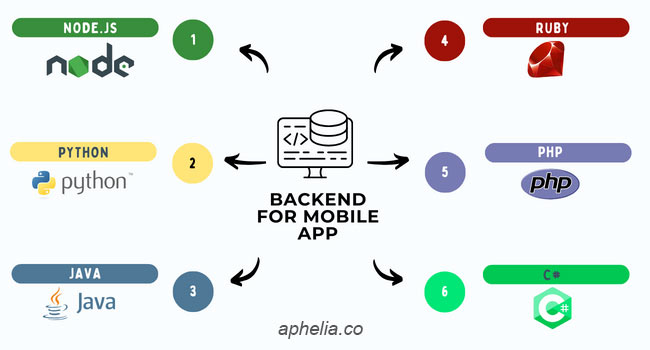
\includegraphics[width=0.75\textwidth]{images/backend_for_mobile_app.jpg}
        \caption{Một số công nghệ phát triển backend cho ứng dụng di động \cite{aphelia2023}.}
        \label{fig:fig1}
      \end{figure}
        \vspace{0.5em}
      
        Về cơ sở dữ liệu, có thể sử dụng các hệ quản trị quan hệ như MySQL hoặc PostgreSQL, tùy theo độ phức tạp của dữ liệu và yêu cầu về hiệu năng. MySQL phù hợp cho các ứng dụng cần tính ổn định cao, trong khi PostgreSQL cung cấp nhiều tính năng nâng cao hơn. Đối với các ứng dụng di động yêu cầu đồng bộ dữ liệu theo thời gian thực, Firebase Firestore là một lựa chọn phù hợp nhờ khả năng cập nhật nhanh và hỗ trợ tốt cho môi trường di động.
      
        \vspace{0.5em}
      
        Phía frontend và mobile, các framework như React Native, Flutter, Swift, và Kotlin là những lựa chọn phổ biến. React Native và Flutter hỗ trợ phát triển ứng dụng đa nền tảng, trong khi Swift và Kotlin là lựa chọn tối ưu cho phát triển ứng dụng gốc trên iOS và Android tương ứng.
      
        \vspace{0.5em}
      
        Cuối cùng, để tự động hóa quy trình triển khai và kiểm thử, các công cụ CI/CD như GitHub Actions hoặc Jenkins thường được tích hợp vào chu trình phát triển phần mềm. CI/CD là viết tắt của Continuous Integration và Continuous Deployment/Delivery, nghĩa là tích hợp liên tục và triển khai liên tục. Trong quy trình này, mã nguồn được kiểm tra, xây dựng và đưa lên môi trường thử nghiệm hoặc sản xuất một cách tự động, giúp phát hiện lỗi sớm và rút ngắn thời gian phát hành phần mềm.
      
   

\section{Lịch sử ngành lập trình di động}
\begin{flushleft}
  \hspace*{0.8cm}Ngành lập trình di động không xuất hiện một cách đột ngột, mà hình thành song song với sự phát triển của điện thoại di động qua từng thời kỳ. Từ những thiết bị to lớn, đắt đỏ và đơn chức năng, đến các smartphone hiện đại với khả năng xử lý mạnh mẽ và đa nhiệm, lập trình di động đã dần trở thành một lĩnh vực quan trọng trong ngành công nghệ thông tin. Việc hiểu rõ bối cảnh và các bước ngoặt trong lịch sử phát triển không chỉ giúp ta nhìn nhận đúng vai trò của lập trình di động, mà còn cho thấy những thách thức và cơ hội trong hành trình tạo ra các ứng dụng phục vụ hàng tỷ người dùng trên toàn cầu.
\end{flushleft}
% 2.1
\subsection{Tổng quan về lịch sử ngành lập trình di động}
\renewcommand{\labelitemi}{--}  

\begin{flushleft}
  \hspace*{0.8cm}Lập trình di động là một lĩnh vực đã phát triển song hành với sự tiến hóa của thiết bị di động trong suốt nhiều thập kỷ. Từ những năm 1990, khi các thiết bị cầm tay đầu tiên như Nokia và BlackBerry bắt đầu phổ biến, nhu cầu về các phần mềm cơ bản như lịch, máy tính và trò chơi đơn giản đã thúc đẩy sự ra đời của các nền tảng lập trình di động ban đầu. Những ứng dụng này chủ yếu được viết bằng ngôn ngữ C hoặc Java ME, giới hạn bởi phần cứng yếu và màn hình nhỏ.
\end{flushleft}

\begin{flushleft}
  \hspace*{0.8cm}Giai đoạn chuyển mình rõ rệt nhất của ngành bắt đầu từ năm 2007, khi Apple giới thiệu iPhone và hệ điều hành iOS. Sự xuất hiện của smartphone với màn hình cảm ứng, kết nối internet mạnh mẽ và kho ứng dụng trực tuyến đã tạo ra một bước ngoặt lớn. Ngay sau đó, Google ra mắt Android – một hệ điều hành mã nguồn mở, cho phép các nhà phát triển dễ dàng tạo ứng dụng và triển khai trên nhiều thiết bị khác nhau.
\end{flushleft}

\begin{flushleft}
  \hspace*{0.8cm}Từ năm 2010 đến nay, lập trình di động đã trở thành một trong những lĩnh vực sôi động nhất của ngành công nghệ thông tin. Các công cụ phát triển như Android Studio, Xcode, cùng với các framework đa nền tảng như React Native, Flutter hay Xamarin, đã giúp rút ngắn thời gian phát triển và mở rộng khả năng tiếp cận người dùng. Đồng thời, những xu hướng mới như trí tuệ nhân tạo (AI), thực tế tăng cường (AR), và Internet vạn vật (IoT) cũng được tích hợp ngày càng sâu vào các ứng dụng di động.
\end{flushleft}

\begin{flushleft}
  \hspace*{0.8cm}Có thể thấy, lịch sử ngành lập trình di động không chỉ phản ánh sự tiến bộ của công nghệ phần cứng và phần mềm, mà còn cho thấy vai trò ngày càng lớn của các ứng dụng trong đời sống hàng ngày. Hiểu rõ bối cảnh lịch sử này là cơ sở quan trọng để các nhà phát triển định hướng tương lai, lựa chọn công cụ phù hợp, và xây dựng các giải pháp sáng tạo đáp ứng nhu cầu người dùng hiện đại.
\end{flushleft}

% 2.2
\subsection{Một số thiết kế của điện thoại di động qua từng thời kỳ}
\renewcommand{\labelitemi}{--}    
    \begin{flushleft}
        \hspace*{0.8cm}Vào những năm 1980, những chiếc điện thoại di động đầu tiên ra đời với thiết kế to, nặng và thường phải mang theo như một chiếc túi xách. Các thiết bị này chủ yếu được sử dụng để nghe và gọi, không có màn hình hiển thị hoặc giao diện tương tác như hiện nay. Lúc này, khái niệm về lập trình di động vẫn chưa xuất hiện vì các thiết bị không hỗ trợ cài đặt thêm phần mềm.
    \end{flushleft}

    \begin{flushleft}
      \hspace*{0.8cm}Đến thập niên 1990, cùng với sự phát triển của công nghệ vi mạch và màn hình LCD, điện thoại di động bắt đầu trở nên nhỏ gọn và phổ biến hơn. Các dòng máy như Nokia 3210 hay Motorola StarTAC không chỉ hỗ trợ gọi điện và nhắn tin, mà còn tích hợp một số ứng dụng đơn giản như đồng hồ báo thức, lịch và trò chơi Snake. Đây là thời kỳ lập trình di động bắt đầu hình thành, chủ yếu dưới dạng các phần mềm nhúng hoặc ứng dụng đơn giản viết bằng ngôn ngữ C hoặc Java ME.
  \end{flushleft}

  \begin{flushleft}
    \hspace*{0.8cm}Giai đoạn tiếp theo bắt đầu từ năm 2007, khi Apple ra mắt iPhone – một thiết bị đánh dấu kỷ nguyên mới của điện thoại thông minh. Với màn hình cảm ứng đa điểm, hiệu năng mạnh mẽ và khả năng kết nối internet, iPhone đã thay đổi hoàn toàn cách người dùng tương tác với thiết bị di động. Sự ra đời của App Store vào năm 2008 đã mở ra một thị trường ứng dụng sôi động, thúc đẩy sự phát triển mạnh mẽ của lập trình di động. Gần như song song, Google cũng phát triển Android – hệ điều hành mã nguồn mở, cho phép các nhà sản xuất và lập trình viên tự do phát triển ứng dụng và tùy biến theo nhu cầu.
\end{flushleft}

\begin{flushleft}
  \hspace*{0.8cm}Từ năm 2010 đến nay, thiết bị di động đã đạt được những bước tiến vượt bậc về hiệu năng, độ phân giải màn hình, dung lượng pin và khả năng xử lý đa nhiệm. Đồng thời, các công nghệ mới như trí tuệ nhân tạo (AI), thực tế ảo (VR), thực tế tăng cường (AR), và cảm biến sinh trắc học cũng được tích hợp ngày càng sâu vào thiết bị. Bên cạnh đó, sự xuất hiện của các nền tảng phát triển đa nền tảng như React Native, Flutter, và Xamarin đã tạo điều kiện thuận lợi cho các nhà phát triển viết ứng dụng một lần và triển khai trên cả iOS lẫn Android.
\end{flushleft}

\begin{flushleft}
  \hspace*{0.8cm}Có thể thấy, thiết bị di động không ngừng được cải tiến cả về phần cứng lẫn phần mềm. Từ một công cụ liên lạc đơn giản, chúng đã trở thành trung tâm của mọi hoạt động số hóa trong đời sống hiện đại – từ học tập, làm việc, giải trí cho đến quản lý tài chính cá nhân. Quá trình phát triển qua các giai đoạn này không chỉ mở ra nhiều cơ hội cho lập trình viên, mà còn đặt ra những thách thức mới về hiệu suất, bảo mật và trải nghiệm người dùng.
\end{flushleft}

% 2.3
\subsection{Motorola DynaTAC 8000X – Bước ngoặt đầu tiên của điện thoại di động}
\renewcommand{\labelitemi}{--}    
\begin{flushleft}
    \hspace*{0.8cm}Motorola DynaTAC 8000X, được giới thiệu vào năm 1983, là chiếc điện thoại di động thương mại đầu tiên trên thế giới. Thiết bị này đã đánh dấu một bước ngoặt quan trọng trong ngành viễn thông toàn cầu khi lần đầu tiên mang lại khả năng liên lạc di động thực sự cho người dùng cá nhân. Với hình dáng to lớn và trọng lượng nặng, DynaTAC vẫn nhanh chóng trở thành biểu tượng công nghệ của thời đại, đặt nền móng cho sự hình thành và phát triển sau này của các thiết bị di động thông minh cũng như ngành lập trình ứng dụng di động.~\cite{motorola1983}
\end{flushleft}

\begin{flushleft}
  \hspace*{0.8cm}DynaTAC 8000X sở hữu thiết kế nổi bật theo phong cách công nghiệp, với kích thước khoảng 33 x 4.4 x 8.9 cm và trọng lượng lên đến 1.1 kg. Người dùng cần sử dụng cả hai tay để thao tác, khiến nó được gọi với biệt danh quen thuộc là “brick phone” – điện thoại cục gạch. Đây là minh chứng rõ rệt cho giai đoạn khởi đầu của công nghệ di động, khi tính cơ động vẫn còn là một khái niệm tương đối.
\end{flushleft}

\begin{flushleft}
  \hspace*{0.8cm}Về mặt kinh tế, thiết bị này là một sản phẩm xa xỉ. Với mức giá lên tới \$3,995 vào năm 1983 (tương đương hơn \$10,000 hiện nay sau điều chỉnh lạm phát), DynaTAC chỉ phù hợp với tầng lớp thượng lưu hoặc những người có nhu cầu đặc biệt. Không chỉ đắt đỏ về giá mua, người dùng còn phải trả thêm chi phí thuê bao hàng tháng và phí gọi tính theo phút – làm cho việc sử dụng thiết bị trở thành một khoản đầu tư lớn về tài chính.
\end{flushleft}

\begin{flushleft}
  \hspace*{0.8cm}Về mặt kỹ thuật, DynaTAC không sở hữu màn hình màu, cảm ứng hay các chức năng nâng cao. Thiết bị chỉ phục vụ chức năng cơ bản là thực hiện và nhận cuộc gọi. Tuy nhiên, chính việc đưa công nghệ viễn thông ra khỏi không gian cố định – như điện thoại bàn – đã mở ra một thời kỳ hoàn toàn mới, trong đó việc giao tiếp trở nên linh hoạt hơn bao giờ hết. Đó là tiền đề quan trọng để những công nghệ di động sau này phát triển mạnh mẽ hơn.
\end{flushleft}

\begin{flushleft}
  \hspace*{0.8cm}Tuy không hỗ trợ cài đặt phần mềm hay ứng dụng, DynaTAC vẫn có vai trò đặc biệt trong lịch sử lập trình di động. Sự xuất hiện của nó đã cho thấy tiềm năng thương mại rất lớn của các thiết bị cầm tay, từ đó thúc đẩy các nhà sản xuất phần cứng và kỹ sư viễn thông đầu tư vào nghiên cứu, phát triển hệ điều hành và nền tảng phần mềm cho thiết bị di động. Nhu cầu mở rộng chức năng thiết bị đã đặt nền móng cho việc phát triển các ứng dụng nhúng đầu tiên và các hệ điều hành cơ bản dành riêng cho di động.
\end{flushleft}

\begin{flushleft}
  \hspace*{0.8cm}Nhìn một cách tổng thể, DynaTAC 8000X không chỉ là thiết bị điện thoại đầu tiên mà còn là biểu tượng khởi đầu của một ngành công nghiệp đầy tiềm năng. Mặc dù giới hạn về công nghệ và chức năng, sự thành công thương mại của nó đã truyền cảm hứng cho hàng loạt phát minh sau này – từ điện thoại thông minh cho tới hệ sinh thái lập trình ứng dụng di động đa dạng và phong phú như hiện nay.
\end{flushleft}

% 2.4
\subsection{Từ “cục gạch” đến trải nghiệm người dùng hiện đại}
\renewcommand{\labelitemi}{--}    
    \begin{flushleft}
        \hspace*{0.8cm}Sau khi điện thoại di động ra đời vào thập niên 1980, công nghệ đã không ngừng tiến hóa để biến những thiết bị vốn to lớn, nặng nề và đắt đỏ thành các sản phẩm nhỏ gọn, tiện lợi và phổ biến trong đời sống hàng ngày. Quá trình thu nhỏ phần cứng đi kèm với việc mở rộng khả năng xử lý và kết nối đã biến điện thoại di động từ một công cụ liên lạc thành một nền tảng công nghệ mạnh mẽ. Trong bối cảnh đó, trải nghiệm người dùng (User Experience – UX) dần trở thành một yếu tố trọng tâm, không chỉ trong thiết kế phần cứng mà còn trong quá trình phát triển phần mềm ứng dụng.
    \end{flushleft}

    \begin{flushleft}
      \hspace*{0.8cm}Sự phát triển của UX trên thiết bị di động gắn liền với sự thay đổi trong hành vi và kỳ vọng của người dùng. Ban đầu, người dùng điện thoại di động chủ yếu mong muốn một thiết bị có thể thực hiện cuộc gọi ổn định và dễ sử dụng. Tuy nhiên, khi điện thoại trở nên phổ biến và chuyển mình thành điện thoại thông minh, người dùng bắt đầu kỳ vọng nhiều hơn: giao diện phải trực quan, tốc độ xử lý nhanh, thao tác mượt mà và trải nghiệm tổng thể phải liền mạch. Chính sự thay đổi về nhận thức và nhu cầu này đã thúc đẩy ngành lập trình di động phải chuyển hướng từ lập trình chức năng đơn thuần sang thiết kế lấy người dùng làm trung tâm.
    \end{flushleft}

    \begin{flushleft}
      \hspace*{0.8cm}Việc điện thoại trở nên dễ tiếp cận hơn là một trong những yếu tố khiến UX trở thành một vấn đề cốt lõi. Nếu như những chiếc điện thoại đầu tiên có giá hàng nghìn đô la và chỉ phục vụ giới doanh nhân, thì ngày nay, người dùng ở mọi độ tuổi và tầng lớp xã hội đều có thể sở hữu ít nhất một thiết bị di động. Khi số lượng người dùng tăng lên, sự đa dạng về nhu cầu, trình độ công nghệ và thị hiếu sử dụng cũng trở nên phong phú hơn. Điều này tạo ra áp lực lớn đối với các nhà phát triển phần mềm, buộc họ phải tạo ra những sản phẩm vừa đơn giản, dễ dùng, vừa đầy đủ chức năng và mang lại cảm giác sử dụng thoải mái.
  \end{flushleft}

  \begin{flushleft}
    \hspace*{0.8cm}Bên cạnh sự thay đổi của người dùng, sự tiến bộ nhanh chóng của phần cứng cũng là một yếu tố không thể bỏ qua. Các thiết bị hiện đại sở hữu màn hình độ phân giải cao, cảm ứng đa điểm, bộ xử lý mạnh, RAM lớn và pin dung lượng cao. Những tiến bộ này mở ra cơ hội cho các nhà phát triển phần mềm thiết kế giao diện ngày càng sinh động, đẹp mắt và tương tác tốt hơn. Nếu như trước đây ứng dụng di động chỉ có thể hiển thị văn bản đơn giản hoặc hình ảnh tĩnh, thì hiện nay, chúng có thể tích hợp video, hiệu ứng chuyển động, phản hồi xúc giác và thậm chí cả trí tuệ nhân tạo để cá nhân hóa trải nghiệm người dùng.
  \end{flushleft}

  \begin{flushleft}
    \hspace*{0.8cm}Sự thay đổi lớn cũng diễn ra trong vai trò của các nhà sản xuất thiết bị di động. Trong giai đoạn đầu, các nhà sản xuất phần cứng thường là những người duy nhất phát triển phần mềm cho thiết bị của họ, từ giao diện người dùng cho đến các chức năng cơ bản. Tuy nhiên, mô hình này nhanh chóng bộc lộ hạn chế khi không thể đáp ứng kịp tốc độ thay đổi của thị trường và nhu cầu người dùng. Đồng thời, các nhà sản xuất cũng không sẵn sàng chia sẻ chi tiết về phần cứng của họ vì lý do bảo mật và cạnh tranh, khiến cho bên thứ ba rất khó tiếp cận và phát triển phần mềm.
  \end{flushleft}

  \begin{flushleft}
    \hspace*{0.8cm}Chính sự bất cập đó đã làm nảy sinh một nhu cầu mới: cần có một lớp trung gian – hay chính xác hơn là một chuẩn kỹ thuật – giúp kết nối phần mềm với phần cứng một cách hiệu quả và an toàn. Các API (Application Programming Interface), SDK (Software Development Kit) và hệ điều hành di động như iOS hay Android đã ra đời nhằm mục đích đó. Chúng đóng vai trò là cầu nối giữa nhà sản xuất thiết bị và cộng đồng lập trình viên, giúp quá trình phát triển phần mềm trở nên dễ dàng hơn mà không cần phải hiểu sâu về kiến trúc phần cứng.
  \end{flushleft}

  \begin{flushleft}
    \hspace*{0.8cm}Một trong những giải pháp mở đầu cho quá trình này là việc sử dụng trình duyệt web di động như một nền tảng để triển khai ứng dụng. Thay vì phát triển phần mềm cài đặt riêng biệt, các lập trình viên bắt đầu tối ưu hóa trang web để hoạt động tốt trên điện thoại. Từ đó, khái niệm “ứng dụng web di động” ra đời, đóng vai trò như bước chuyển tiếp giữa trình duyệt truyền thống và ứng dụng gốc (native app). Những trải nghiệm đầu tiên trên nền tảng web đã đặt nền móng cho việc hình thành tư duy thiết kế giao diện người dùng hiện đại.
  \end{flushleft}

  \begin{flushleft}
    \hspace*{0.8cm}Nhìn chung, sự phát triển của UX trên thiết bị di động không chỉ phản ánh tiến bộ của công nghệ mà còn cho thấy mối liên kết chặt chẽ giữa phần cứng, phần mềm và hành vi người dùng. Việc đặt người dùng làm trung tâm không chỉ là xu hướng tạm thời mà đã trở thành triết lý phát triển cốt lõi trong ngành lập trình di động hiện đại. Từ “cục gạch” thô sơ ngày xưa đến những chiếc điện thoại tinh xảo hiện nay, trải nghiệm người dùng chính là yếu tố quyết định sự thành bại của một sản phẩm trong thời đại số.
  \end{flushleft}

% 2.5
\subsection{Chuẩn WAP – Khởi đầu cho trình duyệt web trên di động}
\renewcommand{\labelitemi}{--}    
\begin{flushleft}
  \hspace*{0.8cm}Trong những năm cuối thập niên 1990 và đầu những năm 2000, khi điện thoại di động bắt đầu được sử dụng rộng rãi trên toàn cầu, nhu cầu truy cập thông tin mọi lúc mọi nơi cũng trở nên cấp thiết. Tuy nhiên, hạ tầng mạng di động ở thời kỳ này lại chưa đủ phát triển: tốc độ kết nối rất chậm, băng thông hạn chế, và độ ổn định thấp. Vì vậy, việc sử dụng các trang web HTML tiêu chuẩn như trên máy tính là điều gần như không khả thi trên thiết bị di động lúc bấy giờ.
  \end{flushleft}
  
  \begin{flushleft}
  \hspace*{0.8cm}Để giải quyết những hạn chế đó, chuẩn WAP – Wireless Application Protocol đã được ra đời như một giải pháp trung gian nhằm hiện thực hóa giấc mơ duyệt web trên thiết bị di động. WAP là một giao thức truyền thông được thiết kế đặc biệt cho môi trường mạng không dây với mục tiêu tạo điều kiện cho các thiết bị di động có thể truy cập, nhận và hiển thị dữ liệu từ các máy chủ web.
  \end{flushleft}
  
  \begin{flushleft}
  \hspace*{0.8cm}Khác với giao thức HTTP vốn được xây dựng cho các máy tính kết nối mạng ổn định và tốc độ cao, WAP được ví như một “phiên bản rút gọn” của HTTP, tối ưu hóa cho việc vận hành trên các thiết bị có tài nguyên phần cứng hạn chế và kết nối mạng chậm như 2G hay GPRS. Nhờ vậy, dù rất đơn giản và sơ khai, WAP đã đóng vai trò như chiếc cầu nối giữa thế giới web truyền thống và thiết bị di động.
  \end{flushleft}
  
  \begin{flushleft}
  \hspace*{0.8cm}Một trong những yếu tố then chốt làm nên hiệu quả của WAP chính là ngôn ngữ đánh dấu WML (Wireless Markup Language). Thay vì sử dụng HTML, vốn quá nặng và phức tạp với các thiết bị di động thời bấy giờ, WML được thiết kế nhẹ hơn nhiều, loại bỏ các yếu tố đồ họa và định dạng phức tạp. Cú pháp của WML khá giống HTML nhưng bị giới hạn về số lượng thẻ và khả năng tương tác. Điều này cho phép hiển thị nội dung văn bản đơn giản như tiêu đề, đoạn văn, và các liên kết mà vẫn đảm bảo tốc độ tải nhanh và khả năng tương thích với phần cứng yếu.
  \end{flushleft}
  
  \begin{flushleft}
  \hspace*{0.8cm}Thêm vào đó, kiến trúc của WAP được xây dựng xoay quanh nguyên tắc tối ưu cho mạng yếu, nhằm giảm thiểu tối đa dữ liệu cần truyền và yêu cầu xử lý phức tạp. Nhờ đó, các thiết bị di động có thể tải và hiển thị nội dung một cách hiệu quả hơn, dù đang hoạt động trong điều kiện mạng không ổn định và băng thông hạn chế.
  \end{flushleft}
  
  \begin{flushleft}
  \hspace*{0.8cm}Trong thời kỳ đầu, nhiều tổ chức và hãng thông tấn đã nhanh chóng nhận ra tiềm năng của WAP và bắt đầu phát triển các phiên bản website hỗ trợ giao thức này. CNN là một trong những đơn vị tiên phong, cung cấp nội dung tin tức thời sự cho người dùng di động thông qua nền tảng WAP. Tương tự, ESPN cũng phát triển phiên bản WAP nhằm cập nhật tỉ số thể thao và thông tin thi đấu cho khán giả thường xuyên di chuyển.
  \end{flushleft}
  
  \begin{flushleft}
  \hspace*{0.8cm}Những ví dụ kể trên là minh chứng rõ ràng cho việc các nhà phát triển ứng dụng web đã bắt đầu chú trọng đến nền tảng di động, dù với rất nhiều giới hạn kỹ thuật so với web truyền thống trên máy tính. Tuy vậy, chính những nỗ lực này đã mở ra một hướng đi mới cho lĩnh vực phát triển ứng dụng – hướng đi mà sau này sẽ trở thành một trụ cột quan trọng trong ngành công nghệ.
  \end{flushleft}
  
  \begin{flushleft}
  \hspace*{0.8cm}Xét về mặt lịch sử và ý nghĩa đối với lập trình di động, WAP có thể được xem là cột mốc đánh dấu sự khởi đầu của khái niệm "ứng dụng web di động". Nhờ vào chuẩn này, các lập trình viên thời kỳ đầu đã có môi trường và công cụ để bắt đầu phát triển nội dung dành riêng cho điện thoại di động, dù chỉ ở mức rất cơ bản.
  \end{flushleft}
  
  \begin{flushleft}
  \hspace*{0.8cm}Không những thế, việc áp dụng WAP còn giúp định hình tư duy thiết kế ứng dụng tối giản, ưu tiên tốc độ và hiệu năng – một nguyên tắc vẫn còn giá trị trong phát triển ứng dụng di động hiện đại. Đồng thời, nó cũng mở ra kỷ nguyên mà điện thoại không chỉ là thiết bị nghe gọi, mà còn là cổng kết nối đến thế giới thông tin số – nơi người dùng có thể cập nhật tin tức, tra cứu thông tin, hay tương tác với nội dung web ở bất cứ đâu.
  \end{flushleft}

% 2.6
\subsection{Sự phát triển của thanh toán di động và bước ngoặt trong lập trình ứng dụng}
\renewcommand{\labelitemi}{--}

\begin{flushleft}
\hspace*{0.8cm}Khi điện thoại di động dần trở thành một phần thiết yếu trong đời sống hàng ngày, nhu cầu không chỉ dừng lại ở liên lạc mà còn mở rộng sang các tiện ích phục vụ tiêu dùng và giải trí. Trong quá trình phát triển đó, một yếu tố có vai trò đặc biệt quan trọng trong việc thúc đẩy sự bùng nổ của ứng dụng di động chính là khả năng thanh toán ngay trên thiết bị.
\end{flushleft}

\begin{flushleft}
\hspace*{0.8cm}Trong những ngày đầu, hình thức thanh toán thông qua SMS (Short Message Service) được xem là giải pháp khả thi nhất, bởi vì hầu hết các điện thoại di động đều hỗ trợ gửi và nhận tin nhắn. Với mô hình này, người dùng chỉ cần gửi tin nhắn đến một đầu số dịch vụ như 8xxx hoặc 6xxx để đổi lại các nội dung số như nhạc chuông, hình nền, hình động hay truyện cười. Khoản phí của tin nhắn này cao hơn nhiều so với tin nhắn thông thường và được tính trực tiếp vào tài khoản di động.
\end{flushleft}

\begin{flushleft}
\hspace*{0.8cm}Những tin nhắn dạng này được gọi là VAS – Value Added Services (dịch vụ giá trị gia tăng), và chính chúng đã đặt nền móng cho mô hình kinh doanh nội dung số trên nền tảng di động. Đây cũng là lần đầu tiên mà lập trình viên có thể kiếm tiền thông qua các ứng dụng hoặc nội dung do họ xây dựng, dù vẫn còn ở dạng rất đơn giản.
\end{flushleft}

\begin{flushleft}
\hspace*{0.8cm}Khi điện thoại phát triển và người dùng ngày càng quen với việc tiêu dùng nội dung số, nhiều hình thức thanh toán khác cũng nhanh chóng ra đời để thay thế hoặc bổ sung cho SMS, tạo điều kiện mở rộng mô hình kinh doanh ứng dụng. Một trong số đó là thẻ cào điện thoại, cho phép người dùng nạp tiền vào tài khoản chính rồi sử dụng số dư này để mua vật phẩm hoặc dịch vụ trong game và ứng dụng.
\end{flushleft}

\begin{flushleft}
\hspace*{0.8cm}Tiếp theo là web charging, một hình thức thanh toán hiện đại hơn, cho phép người dùng mua nội dung trực tiếp trên website hoặc ứng dụng mà không cần can thiệp thủ công. Khi người dùng chọn một dịch vụ trên trình duyệt hoặc trong app, hệ thống sẽ tự động trừ tiền vào tài khoản di động mà không yêu cầu xác nhận nhiều bước. Dù còn hạn chế và dễ phát sinh lỗi, web charging đã cho thấy tiềm năng to lớn của thương mại điện tử di động trong tương lai.
\end{flushleft}

\begin{flushleft}
\hspace*{0.8cm}Mặc dù các hình thức thanh toán kể trên còn đơn giản và chưa được bảo mật cao, nhưng chính chúng đã mở ra cánh cửa đầu tiên cho khái niệm “thanh toán di động”. Từ đó, lập trình viên không chỉ viết ứng dụng phục vụ giải trí mà còn có cơ hội tạo ra giá trị kinh tế thực sự, khuyến khích việc đầu tư bài bản vào thiết kế, trải nghiệm người dùng và chiến lược kiếm tiền.
\end{flushleft}

\begin{flushleft}
\hspace*{0.8cm}Song song với sự phát triển của các mô hình thanh toán, ngành lập trình di động cũng chứng kiến một bước chuyển mình mạnh mẽ. Khi người dùng tăng trưởng nhanh chóng và nhu cầu sử dụng di động vượt xa kỳ vọng, các công ty công nghệ lớn như Apple, Google, và sau này là Samsung, Huawei đã chính thức bước vào cuộc chơi với các hệ điều hành và nền tảng ứng dụng riêng biệt.
\end{flushleft}

\begin{flushleft}
\hspace*{0.8cm}Trước giai đoạn này, lập trình di động vẫn chủ yếu dựa vào nền tảng J2ME (Java 2 Micro Edition) – một môi trường phát triển cực kỳ rối rắm. Các lập trình viên phải đối mặt với hàng loạt thách thức: mỗi dòng điện thoại lại có độ phân giải khác nhau, hệ thống phím bấm không đồng nhất, dung lượng bộ nhớ thấp và phần cứng yếu. Công cụ hỗ trợ thì thiếu thốn, giao diện đơn điệu và không có khả năng tái sử dụng mã nguồn.
\end{flushleft}

\begin{flushleft}
\hspace*{0.8cm}Chỉ đến khi phần cứng của thiết bị di động có bước tiến vượt bậc – với màn hình cảm ứng lớn, bộ xử lý mạnh, bộ nhớ RAM dồi dào, cùng lúc đó là sự xuất hiện của iOS (Swift/Objective-C) và Android (Java/Kotlin) – lập trình viên mới thực sự có cơ hội khai phá sức mạnh của nền tảng di động một cách toàn diện. Giao diện đẹp hơn, tốc độ xử lý nhanh hơn và đặc biệt là hệ sinh thái phát triển (SDK, IDE, kho ứng dụng) đầy đủ và nhất quán, đã tạo ra một cuộc cách mạng trong phát triển ứng dụng.
\end{flushleft}

% 2.7
\subsection{Thị trường di động trên toàn thế giới}
\renewcommand{\labelitemi}{--}    
\begin{flushleft}
  \hspace*{0.8cm}Trước năm 2010, khi khái niệm “smartphone” còn khá mới mẻ với phần lớn người dùng, thị trường điện thoại di động toàn cầu vẫn được dẫn dắt bởi những thương hiệu gắn liền với sự bền bỉ, phổ thông và dễ sử dụng. Nổi bật trong số đó, không ai khác chính là Nokia – “ông vua” không ngai của thời kỳ tiền smartphone.
  \end{flushleft}
  
  \begin{flushleft}
  \hspace*{0.8cm}Nokia đã từng bước định hình trải nghiệm di động cho hàng triệu người dùng trên toàn thế giới, từ những chiếc điện thoại đen trắng cơ bản đến các dòng máy màu, hỗ trợ nhạc chuông đa âm, chơi game Java, cài đặt phần mềm và chụp ảnh. Những model như Nokia 1100, 6300, N70, N95 không chỉ phổ biến mà còn trở thành biểu tượng của một thời kỳ công nghệ giản đơn mà hiệu quả.
  \end{flushleft}
  
  \begin{flushleft}
  \hspace*{0.8cm}Tại Việt Nam, Nokia chiếm trọn niềm tin của người dùng nhờ thiết kế chắc chắn, pin “trâu”, giá thành hợp lý và khả năng hoạt động bền bỉ trong nhiều năm. Sự phổ biến của thương hiệu này mạnh đến mức tên “Nokia” từng được dùng để gọi chung cho bất kỳ chiếc điện thoại nào, dù có thể đó là sản phẩm của hãng khác.
  \end{flushleft}
  
  \begin{flushleft}
  \hspace*{0.8cm}Song song với Nokia, các hãng như Blackberry, Sony Ericsson, Samsung, HTC cũng không ngừng nỗ lực chiếm lĩnh thị phần bằng cách phát triển các hệ điều hành riêng biệt hoặc hợp tác với bên thứ ba để tạo ra sự khác biệt. Một số nền tảng phổ biến lúc bấy giờ gồm:
  \begin{itemize}
  \item Symbian (Nokia)
  \item Blackberry OS (Blackberry)
  \item Windows Mobile, Windows CE (Microsoft)
  \item Palm OS, Linux Mobile, Bada OS (Samsung)
  \end{itemize}
  \end{flushleft}
  
  \begin{flushleft}
  \hspace*{0.8cm}Tuy nhiên, một điểm yếu chung của tất cả các hệ điều hành kể trên chính là sự thiếu thống nhất và không thân thiện với lập trình viên. Mỗi hệ điều hành lại có giao diện riêng, API riêng, ngôn ngữ lập trình và tài liệu khác nhau – gây ra vô vàn khó khăn cho nhà phát triển:
  \begin{itemize}
  \item Trải nghiệm người dùng không đồng đều, giao diện không thống nhất.
  \item Bộ công cụ phát triển (SDK) còn sơ khai, thiếu tính năng và khó tiếp cận.
  \item Không có kho ứng dụng tập trung, dẫn đến việc phân phối phần mềm cực kỳ phức tạp.
  \item[]Điều này khiến phần lớn lập trình viên thời điểm đó vẫn còn thờ ơ hoặc làm việc theo kiểu "cho có", bởi chưa có hệ sinh thái đủ hấp dẫn để đầu tư nghiêm túc.
  \end{itemize}
  \end{flushleft}
  
  \begin{flushleft}
  \hspace*{0.8cm}Mọi thứ chỉ thật sự thay đổi khi Apple chính thức ra mắt iPhone vào năm 2007. Thiết bị này không chỉ là một chiếc điện thoại thông minh đầu tiên theo đúng nghĩa hiện đại, mà còn là bước ngoặt vĩ đại của toàn ngành công nghiệp di động.
  \end{flushleft}
  
  \begin{flushleft}
  \hspace*{0.8cm}Với màn hình cảm ứng đa điểm, thiết kế tinh tế không dùng bàn phím vật lý, hiệu năng mạnh mẽ và hệ điều hành ổn định, iPhone đã đặt ra một chuẩn mực mới cho smartphone. Tuy nhiên, cú hích lớn nhất chỉ đến vào năm 2008, khi App Store chính thức ra đời – nền tảng phân phối ứng dụng tập trung đầu tiên trong lịch sử di động.
  \end{flushleft}
  
  \begin{flushleft}
  \hspace*{0.8cm}App Store không chỉ giúp người dùng dễ dàng tìm kiếm và cài đặt phần mềm, mà còn mở ra cơ hội kinh doanh ứng dụng chuyên nghiệp cho lập trình viên trên toàn thế giới. Với một bộ công cụ phát triển mạnh mẽ, tài liệu hướng dẫn đầy đủ và cộng đồng sôi nổi, iOS SDK đã biến lập trình di động từ một công việc khó khăn, mơ hồ thành một ngành công nghiệp sáng tạo thực thụ.
  \end{flushleft}
  
  \begin{flushleft}
  \hspace*{0.8cm}Kể từ đây, lập trình ứng dụng di động bước sang một kỷ nguyên mới, nơi trải nghiệm người dùng, hiệu năng và hệ sinh thái phát triển đóng vai trò trung tâm. Cuộc đua giữa các nền tảng như iOS và Android cũng bắt đầu, tạo nên một trong những giai đoạn sôi động nhất trong lịch sử công nghệ di động.
  \end{flushleft}

% 2.8
\subsection{Thị trường và sự cạnh tranh trong ngành lập trình di động}
\renewcommand{\labelitemi}{--}    
    \begin{flushleft}
        \hspace*{0.8cm}Khi thị trường thiết bị di động bắt đầu bùng nổ vào đầu thập niên 2010, ba ông lớn công nghệ là Microsoft, Apple và Google đã nhanh chóng bước vào một cuộc cạnh tranh gay gắt nhằm chiếm lĩnh thị phần trong cả phần cứng, hệ điều hành và hệ sinh thái ứng dụng. Mỗi công ty lựa chọn một chiến lược phát triển riêng biệt, qua đó không chỉ định hình diện mạo ngành công nghiệp di động mà còn tác động sâu rộng đến cách thức phát triển ứng dụng di động sau này.
    \end{flushleft}

    \begin{flushleft}
      \hspace*{0.8cm}Trong ba ông lớn, Microsoft là cái tên bước vào cuộc chơi di động với nhiều tham vọng nhưng lại chậm chân. Sau khi nhận ra xu thế bùng nổ của smartphone, Microsoft đã tiến hành một thương vụ lớn vào năm 2013: mua lại bộ phận thiết bị và dịch vụ của Nokia với kỳ vọng tạo ra một hệ sinh thái Windows toàn diện, thống nhất từ máy tính, máy tính bảng đến điện thoại. Triết lý phát triển "Windows Universal Platform" (UWP) – một ứng dụng chạy được trên mọi thiết bị – là nỗ lực nhằm tối ưu trải nghiệm lập trình viên và người dùng. Tuy nhiên, Windows Phone lại xuất hiện quá muộn so với iOS và Android. Kho ứng dụng nghèo nàn, cộng đồng lập trình viên thiếu mặn mà, và mặc dù hệ điều hành này có trải nghiệm mượt mà, nhưng lại thiếu linh hoạt và không thể cá nhân hóa sâu. Kết quả, Windows Phone dần bị người dùng quay lưng và cuối cùng bị khai tử, để lại một bài học sâu sắc về tầm quan trọng của thời điểm gia nhập thị trường và sự linh hoạt trong thích nghi với xu thế công nghệ.
    \end{flushleft}

    \begin{flushleft}
      \hspace*{0.8cm}Ngược lại với Microsoft, Apple là công ty dẫn đầu trong cả trải nghiệm người dùng lẫn xây dựng hệ sinh thái khép kín. Với triết lý thiết kế "từ trong ra ngoài" – nghĩa là kiểm soát cả phần cứng và phần mềm – Apple tạo ra sự đồng bộ, ổn định và an toàn cao cho các thiết bị của mình. iPhone nổi bật với thiết kế tinh tế, hiệu năng mượt mà; hệ điều hành iOS ít lỗi và có tính bảo mật cao; App Store được quản lý chặt chẽ, đảm bảo chất lượng ứng dụng. Đồng thời, Apple luôn chú trọng đến việc hỗ trợ lập trình viên thông qua các công cụ chuyên nghiệp như Xcode, ngôn ngữ Swift và các framework như UIKit hay SwiftUI. Sự nhất quán này giúp Apple duy trì vị thế hàng đầu trong phân khúc smartphone cao cấp và sở hữu lượng người dùng trung thành cao bậc nhất thế giới.
    \end{flushleft}

    \begin{flushleft}
      \hspace*{0.8cm}Về phía Google, chiến lược phát triển của họ xoay quanh triết lý mã nguồn mở, với Android là trung tâm của hệ sinh thái di động. Thay vì sản xuất phần cứng đại trà như Apple, Google phát triển Android như một nền tảng mở, cho phép các nhà sản xuất như Samsung, Xiaomi, Oppo hay Huawei tùy biến và tích hợp hệ điều hành này vào thiết bị của họ. Cách tiếp cận này giúp Android nhanh chóng chiếm lĩnh thị phần toàn cầu. Ban đầu, Android bị phê phán vì tính phân mảnh và kém ổn định, nhưng theo thời gian, Google đã liên tục cải tiến hệ điều hành qua từng phiên bản, siết chặt tiêu chuẩn chất lượng trên Google Play và giới thiệu dòng thiết bị Pixel nhằm kiểm soát tốt hơn trải nghiệm người dùng. Nhờ vào sức mạnh về dữ liệu, trí tuệ nhân tạo và mạng lưới dịch vụ (Gmail, Maps, YouTube...), Google vẫn giữ vững vị thế là trụ cột của ngành di động hiện đại.
    \end{flushleft}

    \begin{flushleft}
      \hspace*{0.8cm}Sự cạnh tranh giữa Microsoft, Apple và Google – ba công ty với ba con đường phát triển khác nhau – không chỉ thúc đẩy đổi mới công nghệ mà còn tạo ra một hệ sinh thái lập trình di động phong phú, đa dạng và không ngừng phát triển. Chính sự đối đầu chiến lược này đã đặt nền móng cho những xu hướng lập trình đa nền tảng ngày nay.
    \end{flushleft}

% 2.9
\subsection{Hai hệ điều hành phổ biến nhất ngày nay: iOS và Android.}
\renewcommand{\labelitemi}{--}   
\begin{flushleft}
  \hspace*{0.8cm}Trong thị trường thiết bị di động hiện nay, iOS và Android là hai hệ điều hành chiếm lĩnh tuyệt đối, đồng thời là nền tảng chủ đạo cho việc phát triển ứng dụng di động trên toàn cầu. Mỗi hệ điều hành mang trong mình triết lý thiết kế, kiến trúc kỹ thuật và hệ sinh thái lập trình riêng, qua đó ảnh hưởng mạnh mẽ đến lựa chọn công cụ và quy trình làm việc của lập trình viên.
\end{flushleft}
    \begin{flushleft}
        \hspace*{0.8cm}iOS là hệ điều hành được phát triển độc quyền bởi Apple, chủ yếu sử dụng trên các thiết bị như iPhone, iPad và iPod Touch. Đặc điểm nổi bật của iOS là sự ổn định, hiệu suất cao và mức độ bảo mật nghiêm ngặt, được đảm bảo bởi quy trình kiểm duyệt ứng dụng chặt chẽ trên App Store. Về mặt lập trình, trước đây iOS sử dụng Objective-C, nhưng kể từ năm 2014, ngôn ngữ Swift – hiện đại, dễ học và tối ưu hóa hiệu năng – đã dần thay thế và trở thành ngôn ngữ chính trong phát triển iOS. Các công cụ hỗ trợ như Xcode đóng vai trò trung tâm trong quá trình phát triển, với khả năng mô phỏng, kiểm thử và tối ưu hóa ứng dụng. Ngoài ra, Apple cung cấp nhiều framework mạnh mẽ như UIKit và SwiftUI để xây dựng giao diện người dùng một cách linh hoạt. Tuy nhiên, do hệ sinh thái đóng, lập trình iOS thường phụ thuộc hoàn toàn vào công cụ và quy định của Apple.
    \end{flushleft}

    \begin{flushleft}
      \hspace*{0.8cm}Android, trái lại, là một hệ điều hành mã nguồn mở do Google phát triển, dựa trên nền tảng Linux. Sự cởi mở trong kiến trúc giúp Android được sử dụng trên hàng trăm thương hiệu thiết bị khác nhau như Samsung, Sony, Xiaomi, hay Oppo, từ đó tạo ra một thị trường đa dạng và cạnh tranh mạnh mẽ. Về ngôn ngữ lập trình, Android ban đầu sử dụng Java, nhưng từ năm 2017, Kotlin đã được Google công nhận là ngôn ngữ chính thức do khả năng viết mã ngắn gọn, an toàn và tương thích tốt với Java. Android Studio là môi trường phát triển tích hợp chủ đạo, cung cấp nhiều công cụ hữu ích như trình giả lập thiết bị, Gradle để quản lý dự án, và Firebase để hỗ trợ backend. Nhờ tính chất mở, Android cho phép các nhà sản xuất tùy chỉnh sâu hệ điều hành, nhưng điều này cũng dẫn đến sự phân mảnh trong trải nghiệm người dùng và thách thức trong kiểm thử ứng dụng.
    \end{flushleft}

    \begin{flushleft}
      \hspace*{0.8cm}Bên cạnh phát triển ứng dụng gốc (native) cho từng hệ điều hành, ngày càng nhiều lập trình viên lựa chọn các công cụ phát triển đa nền tảng để tiết kiệm thời gian và công sức. Các nền tảng như Flutter (Google), React Native (Meta), Xamarin (Microsoft) và Unity (phổ biến trong phát triển game) cho phép viết một lần, chạy trên nhiều hệ điều hành. Cụ thể, Flutter sử dụng ngôn ngữ Dart và nổi bật với hiệu suất mượt mà cùng giao diện đẹp; React Native dựa vào JavaScript, cho phép tái sử dụng logic ứng dụng từ web sang mobile; Xamarin dùng ngôn ngữ C\# để tạo ứng dụng native cho cả iOS lẫn Android; còn Unity, vốn mạnh trong phát triển trò chơi, cũng có thể tạo ra các ứng dụng tương tác cao. Mặc dù các công cụ này mang lại lợi ích về năng suất, nhưng vẫn tồn tại một số hạn chế về hiệu năng và khả năng truy cập đến các API hệ thống sâu.
    \end{flushleft}

    \begin{flushleft}
      \hspace*{0.8cm}Tóm lại, sự phát triển vượt bậc của iOS và Android, cùng với sự ra đời của các công cụ phát triển đa nền tảng, đã tạo nên một môi trường phong phú, năng động và đầy tiềm năng cho ngành lập trình di động. Việc hiểu rõ đặc điểm của từng hệ điều hành và lựa chọn công cụ phù hợp sẽ là yếu tố then chốt giúp lập trình viên tối ưu hóa hiệu quả và chất lượng sản phẩm.
    \end{flushleft}
\section{Tổng quan về các kiến trúc phần mềm}


  \hspace*{0.8cm}Trong quá trình phát triển ứng dụng di động, kiến trúc phần mềm không chỉ đóng vai trò định hình cấu trúc của mã nguồn mà còn ảnh hưởng trực tiếp đến khả năng mở rộng, bảo trì và hiệu suất vận hành của toàn bộ hệ thống. Việc lựa chọn mô hình kiến trúc phù hợp với tính chất của ứng dụng và nền tảng triển khai sẽ giúp các lập trình viên tối ưu quy trình phát triển, đồng thời nâng cao tính linh hoạt và khả năng tái sử dụng của mã nguồn. Trong chương này, chúng ta sẽ lần lượt khảo sát một số mẫu kiến trúc phần mềm phổ biến như mô hình phân lớp (Layers), kiến trúc MVC – thường gặp trên iOS, kiến trúc MVVM – được ưa chuộng trong Android hiện đại, và mô hình giao tiếp Client–Server. Qua đó, chương này nhằm mục tiêu cung cấp cái nhìn toàn diện về cách các kiến trúc phần mềm góp phần vào việc xây dựng những ứng dụng di động ổn định, dễ mở rộng và đáp ứng tốt nhu cầu người dùng.


% 3.1
\subsection{Mẫu kiến trúc Layers}
\renewcommand{\labelitemi}{--}    

    \hspace*{0.8cm}Một trong những mẫu kiến trúc nền tảng và phổ biến nhất trong phát triển phần mềm là kiến trúc phân lớp (Layers). Mô hình này được áp dụng rộng rãi trên cả hai nền tảng iOS và Android do khả năng tổ chức mã nguồn theo hướng tách biệt rõ ràng từng chức năng. Trong kiến trúc Layers, ứng dụng được chia thành ba lớp chính: lớp giao diện (Presentation Layer), lớp xử lý nghiệp vụ (Business Logic Layer), và lớp dữ liệu (Data Layer). Mỗi lớp đảm nhiệm một vai trò riêng biệt, giúp cấu trúc hệ thống trở nên rõ ràng, dễ hiểu và dễ kiểm soát.


% https://viquynh.wordpress.com/2018/02/05/mo-hinh-mvc2-code-demo-jsp-servlet-javabe/
\begin{figure}[H]
    \centering
    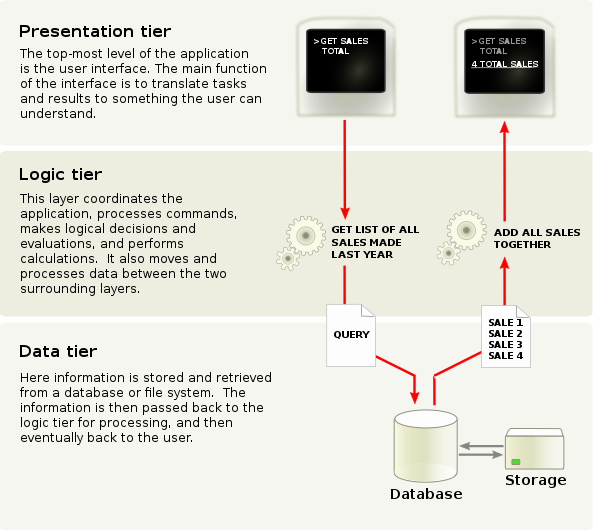
\includegraphics[width=0.66\textwidth]{images/layer.png}
    \caption{Mô hình kiến trúc 3 tầng (3-tiers) \cite{viquynhMVC2}.}
    \label{fig:fig11}
  \end{figure}
    
    
        \hspace*{0.8cm}Cụ thể, lớp Presentation đóng vai trò là điểm tương tác giữa người dùng và hệ thống, chịu trách nhiệm hiển thị thông tin và thu nhận thao tác từ phía người dùng. Lớp Business Logic là nơi xử lý toàn bộ logic nghiệp vụ, từ kiểm tra dữ liệu nhập vào đến các phép tính, xử lý trạng thái và ra quyết định. Cuối cùng, lớp Data đảm nhiệm vai trò giao tiếp với nguồn dữ liệu – có thể là cơ sở dữ liệu cục bộ hoặc server từ xa – và thực hiện các thao tác đọc, ghi hoặc đồng bộ hóa.
    
    
        \vspace{0.5em}
    
        \hspace*{0.8cm}Ưu điểm nổi bật của mô hình Layers là tính phân tách trách nhiệm (separation of concerns). Mỗi lớp chỉ đảm nhiệm một nhóm chức năng chuyên biệt, nên khi có thay đổi hoặc lỗi phát sinh ở một lớp, lập trình viên có thể xử lý mà không ảnh hưởng đến các lớp còn lại. Điều này đặc biệt quan trọng trong các dự án lớn hoặc khi có nhiều lập trình viên cùng tham gia. Ngoài ra, việc kiểm thử (testing) cũng trở nên dễ dàng hơn nhờ tính độc lập giữa các lớp. Tuy nhiên, mô hình này cũng có thể dẫn đến sự phụ thuộc theo chiều dọc giữa các lớp nếu không được thiết kế đúng cách, và đôi khi làm tăng số lượng lớp và khối lượng mã khi ứng dụng phát triển phức tạp hơn.
    
        \vspace{0.5em}
    
        \hspace*{0.8cm}Nhìn chung, kiến trúc phân lớp đóng vai trò như một mô hình nền tảng, thích hợp với nhiều loại ứng dụng khác nhau. Nhờ khả năng tổ chức tốt và dễ mở rộng, mô hình này thường được sử dụng làm cơ sở cho các kiến trúc phức tạp hơn như MVC hay MVVM, đóng góp vào việc xây dựng phần mềm có cấu trúc bền vững và hiệu quả.
    

% 3.2
\subsection{Mẫu kiến trúc MVC}
\renewcommand{\labelitemi}{--}    
    
        \hspace*{0.8cm}Trong số các mô hình kiến trúc phần mềm được áp dụng trên nền tảng iOS, Model View Controller (MVC) là một trong những mô hình lâu đời và phổ biến nhất. MVC chia ứng dụng thành ba thành phần chính, từ đó giúp lập trình viên dễ dàng tổ chức mã nguồn và phân tách nhiệm vụ của từng bộ phận trong quá trình phát triển. Trong đó, thành phần Model đảm nhiệm vai trò quản lý dữ liệu và xử lý các quy tắc nghiệp vụ, đóng vai trò như “bộ não” của ứng dụng. Tiếp theo, thành phần View chịu trách nhiệm hiển thị thông tin tới người dùng, phản ánh đúng trạng thái hiện tại của dữ liệu từ Model. Cuối cùng, thành phần Controller đóng vai trò trung gian, cầu nối giữa View và Model, đảm nhận việc xử lý các sự kiện tương tác của người dùng, đồng thời cập nhật lại giao diện khi dữ liệu thay đổi.
    

    % https://daynhauhoc.com/t/loi-load-du-lieu-len-jsp/109965/10
\begin{figure}[H]
    \centering
    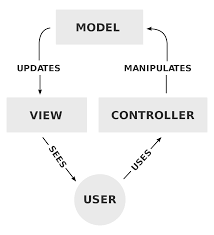
\includegraphics[width=0.44\textwidth]{images/mvc.png}
    \caption{Mô hình kiến trúc MVC \cite{daynhauhocMVC}.}
    \label{fig:fig12}
  \end{figure}

    
      \hspace*{0.8cm}Với cấu trúc như vậy, mô hình MVC mang đến cho lập trình viên iOS một cách tiếp cận đơn giản, dễ hiểu, phù hợp với những người mới bắt đầu tiếp cận lập trình giao diện người dùng. Tuy nhiên, trong thực tế triển khai, một vấn đề lớn phát sinh là hiện tượng “Massive View Controller” \cite{massive_vc}, khi Controller bị quá tải do chứa cả logic giao diện lẫn logic nghiệp vụ. Điều này dẫn đến mã nguồn trở nên khó bảo trì, khó kiểm thử và dễ phát sinh lỗi khi mở rộng chức năng. Chính vì thế, ngày càng nhiều lập trình viên iOS hiện đại chuyển sang các mô hình khác như MVVM hoặc VIPER để giảm thiểu sự phụ thuộc và tách biệt rõ ràng các thành phần chức năng hơn. Nhìn chung, mặc dù MVC vẫn giữ được tính phổ biến nhất định, đặc biệt trong các ứng dụng đơn giản, nhưng nó không còn là lựa chọn tối ưu trong các dự án phức tạp hoặc quy mô lớn.
    

% 3.3
\subsection{Mô hình kiến trúc MVVM}
\renewcommand{\labelitemi}{--}    
    
        \hspace*{0.8cm}Trên nền tảng Android, mô hình kiến trúc Model–View–ViewModel (MVVM) ngày càng trở nên phổ biến nhờ khả năng tương thích cao với các thư viện hỗ trợ hiện đại như LiveData, ViewModel, và Data Binding. MVVM được thiết kế để tách biệt rõ ràng giữa giao diện người dùng và logic nghiệp vụ, đồng thời hỗ trợ tốt cho việc phát triển theo hướng phản ứng (reactive programming). Trong mô hình này, Model tiếp tục đảm nhiệm vai trò quản lý dữ liệu và xử lý các quy tắc nghiệp vụ, tương tự như trong mô hình MVC. View, tức giao diện người dùng, có nhiệm vụ hiển thị dữ liệu và nhận tương tác từ người dùng, tuy nhiên, thay vì xử lý trực tiếp các thao tác đó, View sẽ truyền tín hiệu cho ViewModel để xử lý.
    

    % https://teky.edu.vn/blog/lap-trinh-web-mvc/
\begin{figure}[H]
    \centering
    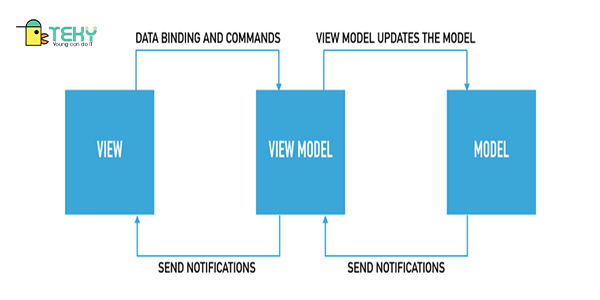
\includegraphics[width=0.67\textwidth]{images/mvvm.jpg}
    \caption{Mô hình kiến trúc MVVM \cite{tekyMVVM}}
    \label{fig:fig13}
  \end{figure}

    
      \hspace*{0.8cm}Thành phần cốt lõi giúp MVVM trở nên nổi bật chính là ViewModel – lớp trung gian giữa View và Model. ViewModel không chứa tham chiếu trực tiếp tới View, mà hoạt động dựa trên cơ chế Observer Pattern, cho phép dữ liệu được quan sát và cập nhật tự động từ ViewModel lên View mỗi khi có thay đổi. Nhờ đó, View trở nên “mỏng” hơn vì chỉ tập trung vào hiển thị, còn toàn bộ logic xử lý sự kiện, tính toán hoặc tương tác với dữ liệu được chuyển giao sang ViewModel. Cách tiếp cận này không những giúp giảm sự ràng buộc giữa các lớp, mà còn tăng khả năng tái sử dụng, kiểm thử tự động và phát triển song song giữa các thành viên trong nhóm \cite{testability_mvvm}.
    
      \vspace{0.5em}
    
        \hspace*{0.8cm}Tóm lại, MVVM phù hợp với xu hướng phát triển ứng dụng hiện đại trên Android khi đặt trọng tâm vào tính phân tách, phản ứng và mở rộng. So với các mô hình truyền thống như MVC, MVVM mang lại kiến trúc rõ ràng hơn và giúp lập trình viên kiểm soát ứng dụng hiệu quả trong cả giai đoạn phát triển lẫn bảo trì.
    

% 3.4
\subsection{Hỗ trợ mô hình Client – Server}
\renewcommand{\labelitemi}{--}    
    
        \hspace*{0.8cm}Trong quá trình xây dựng ứng dụng di động hiện đại, mô hình Client–Server luôn đóng vai trò then chốt trong việc hỗ trợ các chức năng có kết nối mạng. Cả hai nền tảng iOS và Android đều cung cấp đầy đủ công cụ để triển khai mô hình này một cách hiệu quả. Trong mô hình Client–Server, ứng dụng di động đóng vai trò như Client, có nhiệm vụ gửi các yêu cầu (request) tới một máy chủ từ xa (Server) thông qua các giao thức HTTP với các phương thức như GET, POST, PUT, DELET. Sau khi tiếp nhận yêu cầu, Server sẽ xử lý thông tin, truy xuất cơ sở dữ liệu và trả về kết quả dưới dạng JSON hoặc XML để Client hiển thị hoặc xử lý tiếp theo.
    

    % https://codelearn.io/sharing/tim-hieu-ve-mo-hinh-client-server
\begin{figure}[H]
    \centering
    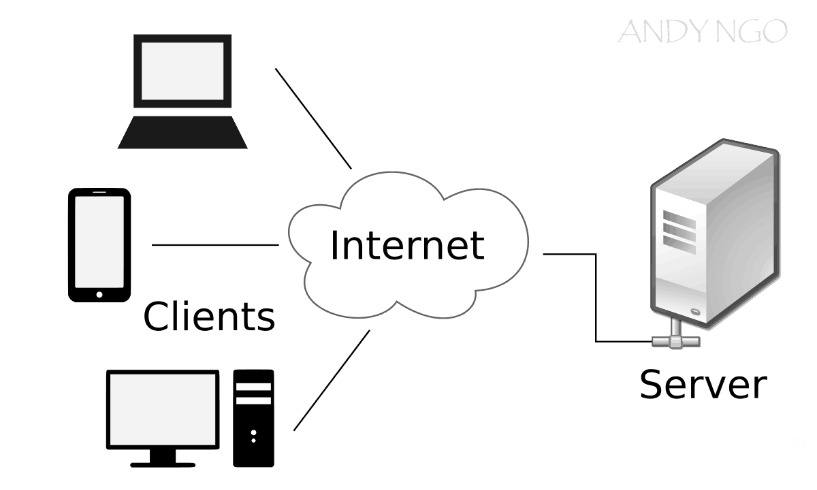
\includegraphics[width=0.75\textwidth]{images/client-server.jpg}
    \caption{Mô hình Client – Server \cite{codelearnClientServer}.}
    \label{fig:fig14}
  \end{figure}

    
      \hspace*{0.8cm}Để hỗ trợ tốt cho mô hình này, các hệ điều hành di động đều cung cấp nhiều thư viện mạnh mẽ. Trên iOS, lập trình viên có thể sử dụng URLSession như một công cụ tiêu chuẩn từ Apple hoặc tích hợp thư viện bên thứ ba như Alamofire để đơn giản hóa các tác vụ mạng. Tương tự, Android cung cấp các thư viện Retrofit và OkHttp giúp việc gửi yêu cầu và xử lý phản hồi trở nên nhanh chóng, dễ mở rộng và dễ kiểm thử. Thông qua mô hình Client–Server, ứng dụng di động có thể hoạt động nhẹ nhàng hơn vì dữ liệu và logic nặng được xử lý ở phía máy chủ. Ngoài ra, tính năng đồng bộ dữ liệu và cập nhật thời gian thực giữa nhiều thiết bị người dùng cũng được hiện thực hóa dễ dàng thông qua mô hình này. Điều này cho thấy Client–Server không chỉ là một mô hình kết nối, mà còn là nền tảng cốt lõi giúp ứng dụng thích ứng linh hoạt trong môi trường đa thiết bị và thay đổi liên tục ngày nay \cite{scalable_mobile_arch}.
    

% 3.5
\subsection{Đánh giá tổng quan}
\renewcommand{\labelitemi}{--}    
    
        \hspace*{0.8cm}Dưới góc nhìn tổng quan, các mô hình kiến trúc phần mềm như MVC, MVVM và Client–Server đều mang đến những giá trị thiết thực trong việc phát triển ứng dụng di động. Tuy nhiên, mỗi nền tảng lại có sự ưu tiên khác nhau trong cách tiếp cận và tổ chức mã nguồn. Đối với nền tảng iOS, mô hình MVC từng được xem là tiêu chuẩn “vàng” nhờ vào sự đơn giản và dễ học. Thế nhưng, hạn chế lớn nhất của MVC – đó là hiện tượng “Massive View Controller” – đã khiến nhiều lập trình viên tìm đến các mô hình thay thế để có được cấu trúc tách biệt và linh hoạt hơn \cite{massive_view_controller}.
    
        \vspace{0.5em}
    
        \hspace*{0.8cm}Trong khi đó, Android hiện đại hóa cách tổ chức ứng dụng thông qua mô hình MVVM, tận dụng sức mạnh từ các thành phần như LiveData, ViewModel và Data Binding. Nhờ vậy, lập trình viên có thể giảm mạnh sự phụ thuộc giữa giao diện và logic nghiệp vụ, đồng thời tối ưu khả năng tái sử dụng và kiểm thử mã nguồn. 

        \vspace{0.5em}
        
        \hspace*{0.8cm}Bên cạnh mô hình kiến trúc, đặc điểm hệ điều hành cũng tác động không nhỏ đến trải nghiệm của lập trình viên trong quá trình phát triển ứng dụng. Trên iOS, sự đồng nhất về phần cứng và phiên bản hệ điều hành giúp giảm thiểu rủi ro phân mảnh, từ đó đơn giản hóa công tác kiểm thử và tối ưu hiệu năng. Tuy nhiên, môi trường phát triển iOS lại yêu cầu lập trình viên phải sử dụng hệ sinh thái phần mềm riêng biệt của Apple như macOS và Xcode, điều này có thể gây bất tiện cho những người không quen thuộc. Ngược lại, Android mở ra không gian phát triển linh hoạt hơn với nhiều lựa chọn công cụ và hệ điều hành, nhưng lại đặt ra thách thức lớn về mặt phân mảnh thiết bị và phiên bản. Lập trình viên Android thường phải kiểm tra ứng dụng trên nhiều cấu hình khác nhau để đảm bảo tính tương thích, đặc biệt là với những ứng dụng cần hiệu năng cao hoặc sử dụng phần cứng chuyên biệt.
        
        \vspace{0.5em}

        \hspace*{0.8cm}Ngoài ra, cả iOS và Android đều đồng thuận trong việc triển khai mô hình Client–Server nhằm tăng khả năng mở rộng, giảm tải cho thiết bị người dùng và hỗ trợ ứng dụng hoạt động ổn định trong môi trường mạng. Việc nắm rõ đặc điểm, ưu điểm cũng như nhược điểm của từng mô hình kiến trúc sẽ giúp lập trình viên không chỉ lựa chọn đúng giải pháp cho từng dự án cụ thể, mà còn góp phần nâng cao hiệu quả phát triển, khả năng bảo trì và mở rộng sản phẩm trong dài hạn.
    

\section{Phân tích chi tiết các kiến trúc phần mềm}

% 
\subsection{Kiến trúc phần mềm ba tầng (Three-tier architecture)}
\renewcommand{\labelitemi}{--}    
    \begin{flushleft}
        \hspace*{0.8cm}Đây là một mô hình tổ chức phần mềm phổ biến, đặc biệt phù hợp với các hệ thống lớn, có khả năng mở rộng và bảo trì lâu dài. Mô hình này phân chia rõ ràng trách nhiệm của từng tầng, từ việc hiển thị, xử lý logic cho đến lưu trữ dữ liệu. Việc áp dụng kiến trúc ba tầng giúp ứng dụng dễ bảo trì, linh hoạt trong mở rộng và tăng khả năng tái sử dụng mã nguồn.
    \end{flushleft}

    \begin{flushleft}
      \hspace*{0.8cm}Kiến trúc ba tầng có thể áp dụng cho nhiều loại ứng dụng khác nhau: từ ứng dụng đơn giản đến phức tạp, từ ứng dụng độc lập đến ứng dụng kết nối mạng. Việc tách biệt ba tầng không chỉ làm cho mã nguồn trở nên rõ ràng hơn mà còn cho phép các nhóm phát triển làm việc độc lập trên từng tầng.
    \end{flushleft}

    \begin{flushleft}
      \hspace*{0.8cm}Tầng trình diễn (Presentation Layer), đây là tầng giao tiếp với người dùng. Chức năng chính của tầng này bao gồm:
      \setlength{\leftmargini}{1.5cm}
      \begin{itemize}
          \item Hiển thị dữ liệu từ tầng nghiệp vụ theo giao diện trực quan.
          \item Nhận lệnh từ người dùng (qua các nút bấm, form, tương tác giao diện).
          \item Không xử lý logic nghiệp vụ, nhờ vậy giao diện có thể dễ dàng tái sử dụng, thay đổi hoặc cập nhật mà không ảnh hưởng đến các tầng khác.
          \item[]$\Rightarrow$ Một lợi ích lớn là khả năng “lắp ghép” lại với các tầng nghiệp vụ khác nhau – giúp cùng một giao diện có thể sử dụng cho nhiều phiên bản khác nhau của hệ thống.
      \end{itemize}
    \end{flushleft}

    \begin{flushleft}
      \hspace*{0.8cm}Tầng nghiệp vụ (Business Logic Layer), tầng này giữ vai trò trung tâm trong hệ thống. Nó thực hiện:
      \setlength{\leftmargini}{1.5cm}
      \begin{itemize}
          \item Chuẩn bị dữ liệu đầu vào để gửi đến tầng dữ liệu.
          \item Chuyển đổi, xử lý dữ liệu nhận về để trả lại cho tầng trình diễn.
          \item Xử lý các lỗi logic hoặc lỗi phản hồi từ tầng dữ liệu.
          \item Áp dụng các quy tắc nghiệp vụ, như kiểm tra hợp lệ, xử lý quy trình.
          \item[]$\Rightarrow$ Tầng này giúp cô lập các xử lý phức tạp khỏi giao diện và dữ liệu, đảm bảo khả năng kiểm thử và bảo trì cao.
      \end{itemize}
    \end{flushleft}

    \begin{flushleft}
      \hspace*{0.8cm}Tầng dữ liệu (Data Layer), là nơi lưu trữ các thông tin quan trọng nhất của ứng dụng:
      \setlength{\leftmargini}{1.5cm}
      \begin{itemize}
          \item Lưu trữ cơ sở dữ liệu (SQL, NoSQL…).
          \item Thực hiện các truy vấn để đảm bảo hiệu năng và độ chính xác cao.
          \item Có thể tích hợp với cơ sở dữ liệu từ xa (server), hệ thống lưu trữ đám mây hoặc tệp cục bộ.
          \item[]$\Rightarrow$ Việc tối ưu tầng dữ liệu giúp cải thiện đáng kể hiệu năng của toàn hệ thống, đặc biệt là trong các ứng dụng có lượng dữ liệu lớn.
      \end{itemize}
    \end{flushleft}

    \begin{flushleft}
      \hspace*{0.8cm}$\Rightarrow$ Kiến trúc ba tầng mang lại lợi ích lớn về mặt tổ chức mã nguồn, bảo trì, kiểm thử và phát triển theo nhóm. Mỗi tầng có trách nhiệm riêng, từ đó giúp ứng dụng dễ mở rộng và thích ứng với thay đổi trong tương lai.
    \end{flushleft}

% 4.2
\subsection{Kiến trúc MVC (Model – View – Controller)}
\renewcommand{\labelitemi}{--}    
    \begin{flushleft}
        \hspace*{0.8cm}MVC (Model – View – Controller) là một mẫu kiến trúc phần mềm cổ điển, phổ biến trong phát triển ứng dụng, đặc biệt là trên nền tảng iOS. Mục tiêu chính của kiến trúc MVC là tách biệt rõ ràng giữa dữ liệu, giao diện và điều khiển xử lý, từ đó giúp ứng dụng dễ bảo trì, mở rộng và nâng cao trải nghiệm người dùng.
    \end{flushleft}

    \begin{flushleft}
      \hspace*{0.8cm}Mô hình này được hình dung như một sơ đồ ba thành phần, mỗi thành phần đảm nhận một vai trò cụ thể:
      \setlength{\leftmargini}{1.5cm}
      \begin{itemize}
          \item Model: Dữ liệu và logic xử lý dữ liệu.
          \item View: Giao diện hiển thị cho người dùng.
          \item Controller: Bộ điều phối, tiếp nhận hành động từ người dùng và điều khiển luồng xử lý.
          \item[]$\Rightarrow$ Ba thành phần hoạt động tách biệt nhưng liên kết chặt chẽ, đảm bảo ứng dụng vận hành trơn tru và dễ dàng điều chỉnh một phần mà không ảnh hưởng đến phần còn lại.
      \end{itemize}
    \end{flushleft}

    \begin{flushleft}
      \hspace*{0.8cm}Model – Mô hình dữ liệu:
      \setlength{\leftmargini}{1.5cm}
      \begin{itemize}
          \item Định danh những gì cần trả về cho người dùng.
          \item Đây là nơi chứa dữ liệu thô, các quy tắc nghiệp vụ và các thao tác xử lý dữ liệu.
          \item Ví dụ: trong một ứng dụng bán hàng, Model chứa thông tin sản phẩm, đơn hàng, người dùng...
      \end{itemize}
    \end{flushleft}

    \begin{flushleft}
      \hspace*{0.8cm}Controller – Bộ điều khiển:
      \setlength{\leftmargini}{1.5cm}
      \begin{itemize}
          \item Tiếp nhận các yêu cầu từ người dùng (qua View).
          \item Thực hiện các truy vấn tài nguyên, gọi các phương thức xử lý trong Model.
          \item Là “bộ não” điều phối mọi hoạt động trong ứng dụng.
      \end{itemize}
    \end{flushleft}

    \begin{flushleft}
      \hspace*{0.8cm}View – Giao diện người dùng:
      \setlength{\leftmargini}{1.5cm}
      \begin{itemize}
          \item Hiển thị dữ liệu dưới dạng dễ hiểu, thân thiện với người dùng.
          \item View không xử lý logic nghiệp vụ, mà chỉ phản hồi lại theo những gì Controller và Model cung cấp.
          \item View sẽ cập nhật nội dung mỗi khi Model thay đổi.
      \end{itemize}
    \end{flushleft}

    \begin{flushleft}
      \hspace*{0.8cm}MVC giúp tách biệt rõ ràng chức năng, dễ dàng phát triển, kiểm thử và bảo trì. Đồng thời cho phép nhiều lập trình viên làm việc song song: người thiết kế giao diện làm View, lập trình viên backend làm Model, còn Controller kết nối hai phần này. Ngoài ra, nó còn có tính tái sử dụng mã nguồn tốt khi một Model có thể được dùng cho nhiều View khác nhau.
    \end{flushleft}

    \begin{flushleft}
      \hspace*{0.8cm}$\Rightarrow$ Mẫu kiến trúc MVC là một giải pháp hiệu quả giúp tổ chức ứng dụng một cách khoa học và linh hoạt. Việc phân chia ứng dụng thành ba thành phần rõ ràng giúp giảm độ phức tạp khi mở rộng, dễ bảo trì, đồng thời nâng cao hiệu quả làm việc nhóm trong quá trình phát triển ứng dụng. Với iOS, MVC vẫn là lựa chọn được ưa chuộng và hỗ trợ tốt trong môi trường phát triển Xcode và Swift.
    \end{flushleft}

% 4.3
\subsection{Kiến trúc MVVM (Model - View - ViewModel)}
\renewcommand{\labelitemi}{--}    
    \begin{flushleft}
        \hspace*{0.8cm}Kiến trúc MVVM (Model – View – ViewModel) là một trong những mẫu thiết kế hiện đại, được áp dụng phổ biến trong phát triển ứng dụng Android (đặc biệt là với sự hỗ trợ từ Jetpack và Kotlin). MVVM ra đời nhằm tối ưu quá trình phát triển ứng dụng bằng cách tách biệt logic hiển thị và logic xử lý, đồng thời tăng tính tự động hóa trong việc cập nhật dữ liệu nhờ cơ chế Data Binding.
    \end{flushleft}

    \begin{flushleft}
      \hspace*{0.8cm}MVVM có cấu trúc gần giống với MVC, nhưng thay vì để Controller điều khiển toàn bộ luồng xử lý, MVVM đưa vào một tầng trung gian là ViewModel – chịu trách nhiệm “kết nối thông minh” giữa dữ liệu (Model) và giao diện (View):
      \setlength{\leftmargini}{1.5cm}
      \begin{itemize}
          \item Tương tự như MVC, View hiển thị dữ liệu, Model chứa dữ liệu và logic xử lý.
          \item Tuy nhiên, Controller được thay thế bằng ViewModel, giúp giảm bớt sự ràng buộc giữa View và Model.
      \end{itemize}
    \end{flushleft}

    \begin{flushleft}
      \hspace*{0.8cm}Model – Dữ liệu và logic xử lý:
      \setlength{\leftmargini}{1.5cm}
      \begin{itemize}
          \item Là nơi lưu trữ các dữ liệu chính của ứng dụng (như thông tin người dùng, sản phẩm...).
          \item Xử lý các nghiệp vụ như tính toán, truy xuất dữ liệu từ cơ sở dữ liệu hoặc API.
          \item Model không trực tiếp liên hệ với View, mà thông qua ViewModel.
      \end{itemize}
    \end{flushleft}

    \begin{flushleft}
      \hspace*{0.8cm}View – Giao diện hiển thị:
      \setlength{\leftmargini}{1.5cm}
      \begin{itemize}
          \item Là phần người dùng tương tác trực tiếp (giao diện ứng dụng).
          \item View trong MVVM không xử lý logic nghiệp vụ mà chỉ phản ánh lại các dữ liệu từ ViewModel.
          \item Nhờ vào Data Binding, View có thể tự động cập nhật khi dữ liệu trong ViewModel thay đổi – giúp giảm mã lặp và tăng hiệu suất phát triển.
      \end{itemize}
    \end{flushleft}

    \begin{flushleft}
      \hspace*{0.8cm}ViewModel – Cầu nối thông minh:
      \setlength{\leftmargini}{1.5cm}
      \begin{itemize}
          \item Chứa các Model và chuẩn bị dữ liệu để hiển thị cho View.
          \item Tạo ra các LiveData hoặc Observable để View có thể theo dõi và tự động cập nhật giao diện khi dữ liệu thay đổi.
          \item Đồng thời, ViewModel cũng xử lý việc truyền dữ liệu từ View sang Model, giúp cập nhật ngược lại khi người dùng nhập liệu hoặc thực hiện thao tác.
      \end{itemize}
    \end{flushleft}

    \begin{flushleft}
      \hspace*{0.8cm}Một điểm mạnh nổi bật của MVVM là cơ chế Data Binding – liên kết dữ liệu hai chiều:
      \setlength{\leftmargini}{1.5cm}
      \begin{itemize}
          \item Khi một đối tượng thuộc nhóm View (như EditText) thay đổi, dữ liệu tương ứng trong ViewModel (hoặc Model) cũng tự động cập nhật.
          \item Ngược lại, khi ViewModel thay đổi giá trị, View cũng cập nhật lại ngay lập tức.
          \item[]$\Rightarrow$ Điều này giúp hạn chế lỗi khi cập nhật giao diện và rút ngắn thời gian phát triển, đặc biệt là trong các ứng dụng có nhiều thao tác tương tác dữ liệu.
      \end{itemize}
    \end{flushleft}

    \begin{flushleft}
      \hspace*{0.8cm}$\Rightarrow$ MVVM là một mô hình kiến trúc mạnh mẽ, phù hợp với các ứng dụng hiện đại cần cập nhật giao diện linh hoạt, liên tục. Với sự hỗ trợ từ Data Binding và LiveData (trong Android), ViewModel giúp đơn giản hóa việc xử lý dữ liệu và đồng bộ giao diện, đồng thời giảm sự phụ thuộc giữa các thành phần, nâng cao khả năng bảo trì và mở rộng về sau. MVVM hiện là lựa chọn ưu tiên trong các dự án Android có quy mô từ vừa đến lớn.
    \end{flushleft}

% 4.4
\subsection{Kiến trúc Client/Server}
\renewcommand{\labelitemi}{--}    
    \begin{flushleft}
        \hspace*{0.8cm}Trong thời đại số, đa số các ứng dụng cần trao đổi dữ liệu qua Internet. Mô hình Client/Server trở thành kiến trúc không thể thiếu, đặc biệt với các ứng dụng có tính năng đồng bộ dữ liệu, chia sẻ thông tin theo thời gian thực, hoặc sử dụng tài nguyên trên máy chủ từ xa. Đồng thời, cần kết hợp với các kiến trúc nội bộ như MVC hoặc MVVM để tối ưu hóa việc xây dựng giao diện và xử lý logic.
    \end{flushleft}

    \begin{flushleft}
      \hspace*{0.8cm}Kiến trúc Client/Server mô tả mô hình trong đó ứng dụng Client (thiết bị người dùng) gửi yêu cầu đến Server (máy chủ từ xa), thường qua HTTP Request, WebSocket, hoặc Web Service. Các chức năng chính bao gồm:
      \setlength{\leftmargini}{1.5cm}
      \begin{itemize}
          \item Client: Gửi yêu cầu (request), hiển thị dữ liệu, tương tác với người dùng.
          \item Server: Xử lý yêu cầu, truy cập cơ sở dữ liệu, trả về dữ liệu kết quả.
          \item[]$\Rightarrow$ Kiến trúc này phù hợp cho các ứng dụng có nhiều người dùng, cần chia sẻ dữ liệu như mạng xã hội, ứng dụng ngân hàng, thương mại điện tử…
      \end{itemize}
    \end{flushleft}
\section{Các yếu tố ảnh hưởng đến chi phí phát triển ứng dụng}

  Chi phí phát triển ứng dụng là một yếu tố quan trọng mà các doanh nghiệp cần cân nhắc kỹ lưỡng trước khi triển khai dự án phần mềm. Trong thực tế, chi phí này không chỉ phụ thuộc vào quy mô hay mục tiêu của sản phẩm, mà còn bị chi phối bởi nhiều yếu tố kỹ thuật và chiến lược khác nhau. Từ đặc điểm của tính năng, kiến trúc hạ tầng, đến vị trí địa lý của đội ngũ phát triển, mỗi yếu tố đều có thể tạo ra sự chênh lệch đáng kể về ngân sách đầu tư. Phần này sẽ trình bày hai nhóm nội dung chính: (1) các yếu tố cốt lõi tác động đến chi phí xây dựng và duy trì ứng dụng, và (2) sự khác biệt về chi phí nhân sự theo khu vực địa lý trên thế giới. Qua đó, doanh nghiệp có thể xác định các điểm cần ưu tiên, tối ưu nguồn lực và lựa chọn chiến lược phát triển phù hợp với điều kiện thực tế của mình.

  
  
% 5.1
\subsection{Các yếu tố chính ảnh hưởng đến chi phí phát triển ứng dụng}
\renewcommand{\labelitemi}{--}  

% https://assets.goodfirms.co/pdfs/how-much-does-it-cost-to-develop-an-app.pdf
  \begin{figure}[H]
    \centering
    
\includegraphics[width=0.6\textwidth]{images/appCosst.png}
    \caption{Các yếu tố chính ảnh hưởng đến chi phí phát triển ứng dụng \cite{goodfirmsAppCost}.}
    \label{fig:fig20}
  \end{figure}

    
      Trong quá trình phát triển ứng dụng, nhiều yếu tố đóng vai trò quyết định đến tổng chi phí, cả trong giai đoạn thiết kế lẫn sau triển khai. Các yếu tố chính bao gồm:
      \setlength{\leftmargini}{1.5cm}
      \begin{itemize}
          \item Tính năng và chức năng (Features and Functionality): Mức độ phức tạp của tính năng tỷ lệ thuận với chi phí phát triển. Ứng dụng có càng nhiều chức năng nâng cao như định vị, livestream, AI tích hợp,… thì đòi hỏi nguồn lực phát triển cao hơn.
          \item Hạ tầng ứng dụng (App Infrastructure): Cách tổ chức hệ thống backend, tích hợp API, hệ thống lưu trữ dữ liệu, bảo mật và tối ưu hiệu năng đều ảnh hưởng lớn đến ngân sách đầu tư. Hạ tầng vững chắc đảm bảo tính ổn định và khả năng mở rộng lâu dài.
          \item Độ phức tạp của ứng dụng (App Complexity): Mức độ phức tạp trong luồng xử lý nghiệp vụ và logic kinh doanh đòi hỏi thời gian phân tích và phát triển dài hơn, từ đó làm tăng chi phí.
          \item Thiết kế trải nghiệm người dùng (UX/UI Design): Giao diện càng trực quan, hiện đại, và thân thiện thì cần đầu tư nhiều thời gian hơn cho thiết kế và kiểm thử.
          \item Chi phí bảo trì (App Maintenance): Sau khi triển khai, ứng dụng cần cập nhật thường xuyên để vá lỗi, cải tiến tính năng hoặc thích nghi với nền tảng mới.
          \item Yêu cầu bảo mật (App Security): Ứng dụng xử lý dữ liệu nhạy cảm (ngân hàng, y tế, tài chính...) đòi hỏi mức độ bảo mật cao, từ đó làm tăng chi phí đầu tư.
          \item Loại ứng dụng (App Category): Tùy thuộc vào lĩnh vực hoạt động (thương mại điện tử, chăm sóc sức khỏe, mạng xã hội…), mức độ phức tạp và chi phí phát triển sẽ khác nhau.
          \item Số lượng nền tảng và màn hình (Number of Platforms \& Pages): Ứng dụng hỗ trợ nhiều nền tảng như iOS, Android, Web với giao diện đa dạng sẽ phát sinh thêm chi phí thiết kế và kiểm thử.
          \item Vị trí nhóm phát triển (Location of the Development Team): Chi phí nhân công thay đổi theo từng khu vực địa lý. Các nhóm tại Mỹ hoặc Tây Âu thường có chi phí cao hơn so với châu Á.
      \end{itemize}
    \vspace{0.5em}

    
      Trong số các yếu tố trên, kiến trúc hạ tầng phần mềm (App Infrastructure) đóng vai trò then chốt:
      \setlength{\leftmargini}{1.5cm}
      \begin{itemize}
          \item Đây là “xương sống” kỹ thuật của toàn bộ hệ thống, quyết định tính ổn định, bảo mật, khả năng tích hợp API, cloud và cơ sở dữ liệu.
          \item Nếu được thiết kế tốt ngay từ đầu, hạ tầng giúp giảm đáng kể chi phí bảo trì và tránh rủi ro gián đoạn trong quá trình vận hành.
      \end{itemize}
    \vspace{0.5em}

% 5.2
\subsection{Chi phí thuê nhân sự theo khu vực địa lý}

\begin{table}[ht]
  \centering
  \begin{tabular}{|l|c|c|c|c|}
  \hline
  \textbf{Title of Employee} & \textbf{United States} & \textbf{Latin America} & \textbf{Eastern Europe} & \textbf{Asia} \\
  \hline
  Business Analyst    & \$110 -- \$205 & \$45 -- \$55 & \$40 -- \$63 & \$30 -- \$42 \\
  Architect           & \$198 -- \$292 & \$60 -- \$72 & \$50 -- \$77 & \$35 -- \$48 \\
  Project Manager     & \$133 -- \$233 & \$55 -- \$66 & \$45 -- \$70 & \$35 -- \$48 \\
  Jr. Developer       & \$105 -- \$111 & \$35 -- \$44 & \$25 -- \$42 & \$18 -- \$24 \\
  Mid-Level Developer & \$132 -- \$140 & \$30 -- \$52 & \$35 -- \$49 & \$25 -- \$34 \\
  Sr. Developer       & \$154 -- \$163 & \$45 -- \$55 & \$45 -- \$70 & \$30 -- \$42 \\
  Lead Developer      & \$176 -- \$187 & \$50 -- \$61 & \$45 -- \$70 & \$35 -- \$50 \\
  Junior QA           & \$77 -- \$81   & \$30 -- \$39 & \$25 -- \$42 & \$20 -- \$30 \\
  Mid-Level QA        & \$99 -- \$105  & \$35 -- \$44 & \$30 -- \$48 & \$25 -- \$32 \\
  Senior QA           & \$143 -- \$169 & \$40 -- \$51 & \$35 -- \$60 & \$30 -- \$40 \\
  Graphic Designer    & \$79 -- \$163  & \$40 -- \$50 & \$35 -- \$56 & \$25 -- \$36 \\
  \hline
  \end{tabular}
  \caption{Mức lương cho các vai trò nhân viên khác nhau trên khắp các khu vực \cite{rubygarageWebCost}.}
  \label{tab:salary-comparison}
  \end{table}
  
\renewcommand{\labelitemi}{--}    
    
        Một trong những yếu tố quan trọng ảnh hưởng đến tổng chi phí phát triển phần mềm chính là chi phí thuê nhân sự theo khu vực địa lý. Các công ty phần mềm, đặc biệt là những doanh nghiệp quốc tế hoặc các dự án có nhu cầu thuê ngoài (outsourcing), thường căn cứ vào mức chi phí trung bình theo giờ làm việc của các vai trò chuyên môn trong ngành công nghệ thông tin để ra quyết định tuyển dụng. Dữ liệu trong bảng ở phần trên được tổng hợp từ 4 khu vực tiêu biểu trên toàn cầu gồm United States (Hoa Kỳ), Latin America (Mỹ Latin), Eastern Europe (Đông Âu) và Asia (Châu Á). Mỗi khu vực có mức chi phí khác nhau rõ rệt, phản ánh sự chênh lệch về mức sống, kỹ năng lao động cũng như nhu cầu thị trường. Thống kê này bao phủ 12 vai trò phổ biến trong các dự án phát triển phần mềm hiện nay, giúp đưa ra cái nhìn tổng quan về chi phí nhân sự theo từng nhóm chức năng.
    \vspace{0.5em}

    
      Đối với nhóm Quản lý và Thiết kế Kiến trúc, mức chi phí thuê nhân sự được ghi nhận là cao nhất trong tất cả các vai trò. Nhóm này bao gồm ba vị trí chủ chốt: Business Analyst (chuyên viên phân tích nghiệp vụ), Architect (kiến trúc sư phần mềm), và Project Manager (quản lý dự án). Trong đó, kiến trúc sư phần mềm đóng vai trò xây dựng khung nền kỹ thuật, đảm bảo hệ thống có thể mở rộng và vận hành ổn định; còn chuyên viên phân tích nghiệp vụ đóng vai trò cầu nối giữa khách hàng và nhóm kỹ thuật; trong khi quản lý dự án là người điều phối toàn bộ tiến độ và tài nguyên. Tại Hoa Kỳ, mức giá thuê cho các vị trí này có thể lên tới gần \$300/giờ – một con số phản ánh tầm quan trọng chiến lược và yêu cầu chuyên môn cao. Mức chi phí này giảm dần tại các khu vực khác, với Latin America và Eastern Europe dao động ở mức trung bình, còn Asia (Châu Á) là nơi có mức chi phí thấp nhất, chỉ từ \$30 – \$48/giờ. Điều này khiến các công ty quốc tế thường ưu tiên thuê ngoài nhóm nhân sự cấp cao từ khu vực châu Á để tiết kiệm chi phí nhưng vẫn đảm bảo hiệu quả.
    \vspace{0.5em}

    
      Tiếp theo là nhóm Lập trình viên (Developer), một trong những thành phần cốt lõi tạo nên sản phẩm phần mềm. Nhóm này được chia nhỏ theo cấp độ kinh nghiệm, bao gồm: Junior Developer, Mid-Level Developer, Senior Developer và Lead Developer. Sự phân loại này phản ánh mức độ độc lập, độ phức tạp của nhiệm vụ mà mỗi cấp độ có thể đảm nhiệm, cũng như ảnh hưởng đến tiến độ và chất lượng sản phẩm. Mức chi phí thuê sẽ tăng tương ứng với cấp độ, từ Junior đến Lead Developer. Tại các khu vực phát triển như Hoa Kỳ, mức lương của Senior hoặc Lead Developer có thể gần tương đương với nhóm kiến trúc sư. Trong khi đó, các khu vực như Latin America hay Eastern Europe có mức chi phí trung bình, phù hợp cho các công ty tầm trung. Asia tiếp tục là khu vực có lợi thế về chi phí, khi mức thuê nhân sự lập trình ở mọi cấp độ đều ở mức thấp hơn đáng kể, giúp các doanh nghiệp tiết kiệm ngân sách mà vẫn có thể tiếp cận với nguồn lực kỹ thuật chất lượng nếu tuyển chọn kỹ lưỡng.
    \vspace{0.5em}

    
      Trong chu trình phát triển phần mềm, kiểm thử phần mềm (QA) là khâu đảm bảo chất lượng đầu ra trước khi triển khai chính thức. Nhóm QA cũng được chia theo cấp độ kinh nghiệm, bao gồm: Junior QA, Mid-Level QA, và Senior QA. So với Developer hoặc Architect, mức chi phí thuê QA thường thấp hơn, nhưng vẫn có sự chênh lệch rõ rệt giữa các khu vực. Tại Mỹ, một Senior QA có thể nhận mức thù lao lên đến \$169/giờ – thậm chí cao hơn Mid-Level Developer tại cùng khu vực (khoảng \$140/giờ). Điều này cho thấy, tại các thị trường phát triển, việc kiểm thử phần mềm được đánh giá rất cao và đòi hỏi kỹ năng chuyên môn sâu. Tại châu Á, các vai trò QA được thuê với mức giá thấp hơn đáng kể, giúp tiết kiệm đáng kể chi phí cho các công ty đang hướng đến tự động hóa kiểm thử hoặc mở rộng nhóm QA.
    \vspace{0.5em}

    
      Cuối cùng là vai trò thiết kế giao diện (Graphic Designer), vốn không yêu cầu chuyên môn kỹ thuật quá sâu như lập trình nhưng vẫn đóng vai trò quan trọng trong việc tạo ra trải nghiệm người dùng hấp dẫn và nhất quán. Tại các thị trường phát triển như Mỹ, chi phí thuê designer vẫn ở mức khá cao do đòi hỏi về thẩm mỹ, khả năng sử dụng công cụ thiết kế chuyên nghiệp và phối hợp chặt chẽ với nhóm phát triển sản phẩm. Trong khi đó, các khu vực như Đông Âu hay châu Á có chi phí thuê thấp hơn đáng kể, đặc biệt phù hợp với các dự án cần thiết kế giao diện ở mức cơ bản đến trung cấp. Việc lựa chọn graphic designer từ các khu vực này giúp doanh nghiệp duy trì ngân sách ở mức hợp lý mà vẫn đảm bảo tính thẩm mỹ và hiệu quả trong giao diện người dùng.
    \vspace{0.5em}

    
      Tóm lại, chi phí thuê nhân sự phát triển phần mềm có sự biến động lớn theo từng khu vực địa lý và vai trò cụ thể. Việc hiểu rõ mức giá trung bình theo giờ và sự khác biệt giữa các nhóm chuyên môn sẽ giúp doanh nghiệp đưa ra chiến lược thuê nhân sự hiệu quả hơn, cân bằng giữa chi phí và chất lượng. Trong bối cảnh toàn cầu hóa và sự phát triển mạnh mẽ của mô hình làm việc từ xa, các công ty hoàn toàn có thể tối ưu hóa nguồn lực bằng cách kết hợp nhân sự ở các khu vực khác nhau, tận dụng lợi thế chi phí của khu vực châu Á và chất lượng kỹ thuật cao từ các khu vực khác để xây dựng đội ngũ phát triển linh hoạt và hiệu quả.




